%\documentclass{beamer}
\documentclass[handout]{beamer}

\usepackage[utf8]{inputenc}

\usepackage{graphicx}
\usepackage{ifthen}

\usepackage{xcolor}
\usepackage{listings}

\usepackage{tikz}

\usepackage{url}

\usetheme[secheader]{Boadilla}
\usecolortheme{dolphin}

% Main color
\definecolor{grin}{HTML}{0D78B9}
\definecolor{redd}{HTML}{b82200}
\definecolor{uait}{HTML}{ffffff}
\definecolor{blec}{HTML}{000000}


% Colors
\setbeamercolor*{block body}{bg=normal text.bg!93!grin}
\setbeamercolor*{block title}{bg=grin!25!uait}

\setbeamercolor{normal text}{fg=blec!65!grin,bg=uait}

\setbeamercolor{section in toc}{fg=grin}
\setbeamercolor{subsection in toc}{fg=grin!90!uait}

\setbeamercolor{frametitle}{fg=grin,bg=grin!20}

\setbeamercolor*{palette primary}{use=structure,fg=blec,bg=grin!40!uait}
\setbeamercolor*{palette secondary}{use=structure,fg=uait,bg=grin!60!uait}
\setbeamercolor*{palette tertiary}{use=structure,fg=uait,bg=grin!90!uait}
\setbeamercolor*{palette quaternary}{fg=uait,bg=blec}

\setbeamercolor*{sidebar}{use=structure,bg=grin}

\setbeamercolor*{palette sidebar primary}{use=structure,fg=grin!10}
\setbeamercolor*{palette sidebar secondary}{fg=grin!10!uait}
\setbeamercolor*{palette sidebar tertiary}{use=structure,fg=grin!50}
\setbeamercolor*{palette sidebar quaternary}{fg=grin!5!uait}

% Section balls
\setbeamerfont{section number projected}{family=\rmfamily,series=\bfseries,size=\normalsize}
\setbeamercolor{section number projected}{bg=grin!70!uait,fg=uait}

% Itemize balls
\setbeamercolor{item projected}{bg=grin!70!uait}
\setbeamercolor{subitem projected}{bg=grin!90!uait}

% Title
\setbeamercolor*{titlelike}{use=structure,fg=grin}
%lst colors

\definecolor{commentgreen}{RGB}{162, 249, 103}
\definecolor{eminence}{RGB}{108,48,130}
\definecolor{weborange}{RGB}{255,165,0}
\definecolor{frenchplum}{RGB}{254,215,0}
\definecolor{goodred}{RGB}{233, 38, 95}
\definecolor{washedyellow}{RGB}{223, 206, 94}
\definecolor{monoblue}{RGB}{79, 201, 232}

% blue code background
\lstset{
    language=c++,
    frame=single,
    framerule=0pt,
    backgroundcolor=\color{grin!70!blec},
   % basicstyle=\ttfamily\color{white},
    xleftmargin=4.3pt,
    xrightmargin=4.3pt,
    commentstyle=\color{commentgreen},
    stringstyle=\color{washedyellow},
    basicstyle=\small\ttfamily\color{white}, % basic font setting
    keywordstyle = \color{eminence},
    keywordstyle = [2]{\color{weborange}},
    keywordstyle = [3]{\color{monoblue}},
    otherkeywords = {>,<,;,.,-,!,=,~,memcpy,send_request_cgi,encoded,gsub},
    morekeywords = [2]{>,<,;,.,-,!,=,~},
    morekeywords = [3]{memcpy,send_request_cgi,encoded,gsub},
    %emph={int,char,double,float,unsigned,void,bool},
    %emphstyle={\color{blue}},
    escapechar=\&
}


% transparent bg
\setbeamercovered{transparent}

\setbeameroption{show notes}

% tikz round photos
\newcommand{\roundpic}[4][]{
	\tikz\node [circle, minimum width = #2,
		path picture = {
				\node [#1] at (path picture bounding box.center) {
					\includegraphics[width=#3]{#4}};
			}] {};}

% Header slide
\title[Metasploit 1]
{Penetration testing\\Metasploit 1}

\subtitle{Introduction, basics and first exercises}

\author[Group 5]{%
	\texorpdfstring{%
		\begin{columns}
			\column{.33\linewidth}
			\centering
			Paolo Chistè
			\column{.34\linewidth}
			\centering
			Claudio Facchinetti
			\column{.33\linewidth}
			\centering
			Matteo Franzil
		\end{columns}
	}{Group 5}
}

\institute[Chistè, Facchinetti, Franzil]{
	\texorpdfstring{%
		
\includegraphics[width=.6\textwidth]{../drawable/logos/logo-disi.png}
	}{University of Trento}\\
	\smallskip
	%\hphantom{...}\\
	Master's Course in Computer Science
}

\date[19/05/2021]{19 May 2021}

% Indice tra sezioni
\AtBeginSection[]
{
	\begin{frame}
		\frametitle{Summary}
		\tableofcontents[currentsection]
	\end{frame}
}

\begin{document}

% (1) Title page
\frame{\titlepage}

% (2) Introduction
\section{Introduction}

% (3)
\begin{frame}
	\frametitle{Legal disclaimer}

	\onslide<1->{
		The tools outlined in this laboratory lesson may be only used within this lab or other VMs in your own environment. Any use of the framework outside the course may be penalty relevant (i.e. a crime). You are not allowed to apply these attacks to deployed systems unless explicitly authorized to do so.
		\medskip
	}

	\onslide<2->{
		The infrastructure provided is deliberately isolated from the rest of your machine, with no outside-facing virtual adapters. Any modifications made to the network setup is done at your own risk (e.g. inadvertently mounting an attack on one’s own host).
		\medskip
	}
\end{frame}

% (4)
\begin{frame}
    \frametitle{Contents}
    
    All the contents shown here and in the report are available, under the MIT license, on GitHub:
    
    \begin{figure}[h]
		\centering
		
\includegraphics[width=0.3\textwidth]{../drawable/logos/github-logo.png}
	\end{figure}
	
	\begin{center}
	    \url{https://github.com/mfranzil/unitn-m-ns}
	\end{center}
\end{frame}


% (4)
\begin{frame}
	\frametitle{Introduction}

	What is \textbf{penetration testing}?

	\onslide<1->{
		\begin{block}{Wikipedia}
			A penetration test [...] is an authorized simulated cyberattack on a computer system, performed to evaluate the security of the system; this is not to be confused with a \textit{vulnerability assessment}. The test is performed to identify [...] vulnerabilities, including \textbf{the potential for unauthorized parties to gain access to the system's features and data} [...].
		\end{block}
	}

	\onslide<2->{
		\begin{block}{Cloudflare}
			Penetration testing (or pen testing) is a security exercise where a cyber-security expert attempts to find and exploit vulnerabilities in a computer system. The purpose of this simulated attack is to \textbf{identify any weak spots} in a system’s defenses which attackers could take advantage of.
		\end{block}
	}
\end{frame}

% (5)
\begin{frame}
	\frametitle{Penetration testing}

	\begin{figure}[h]
		\centering
		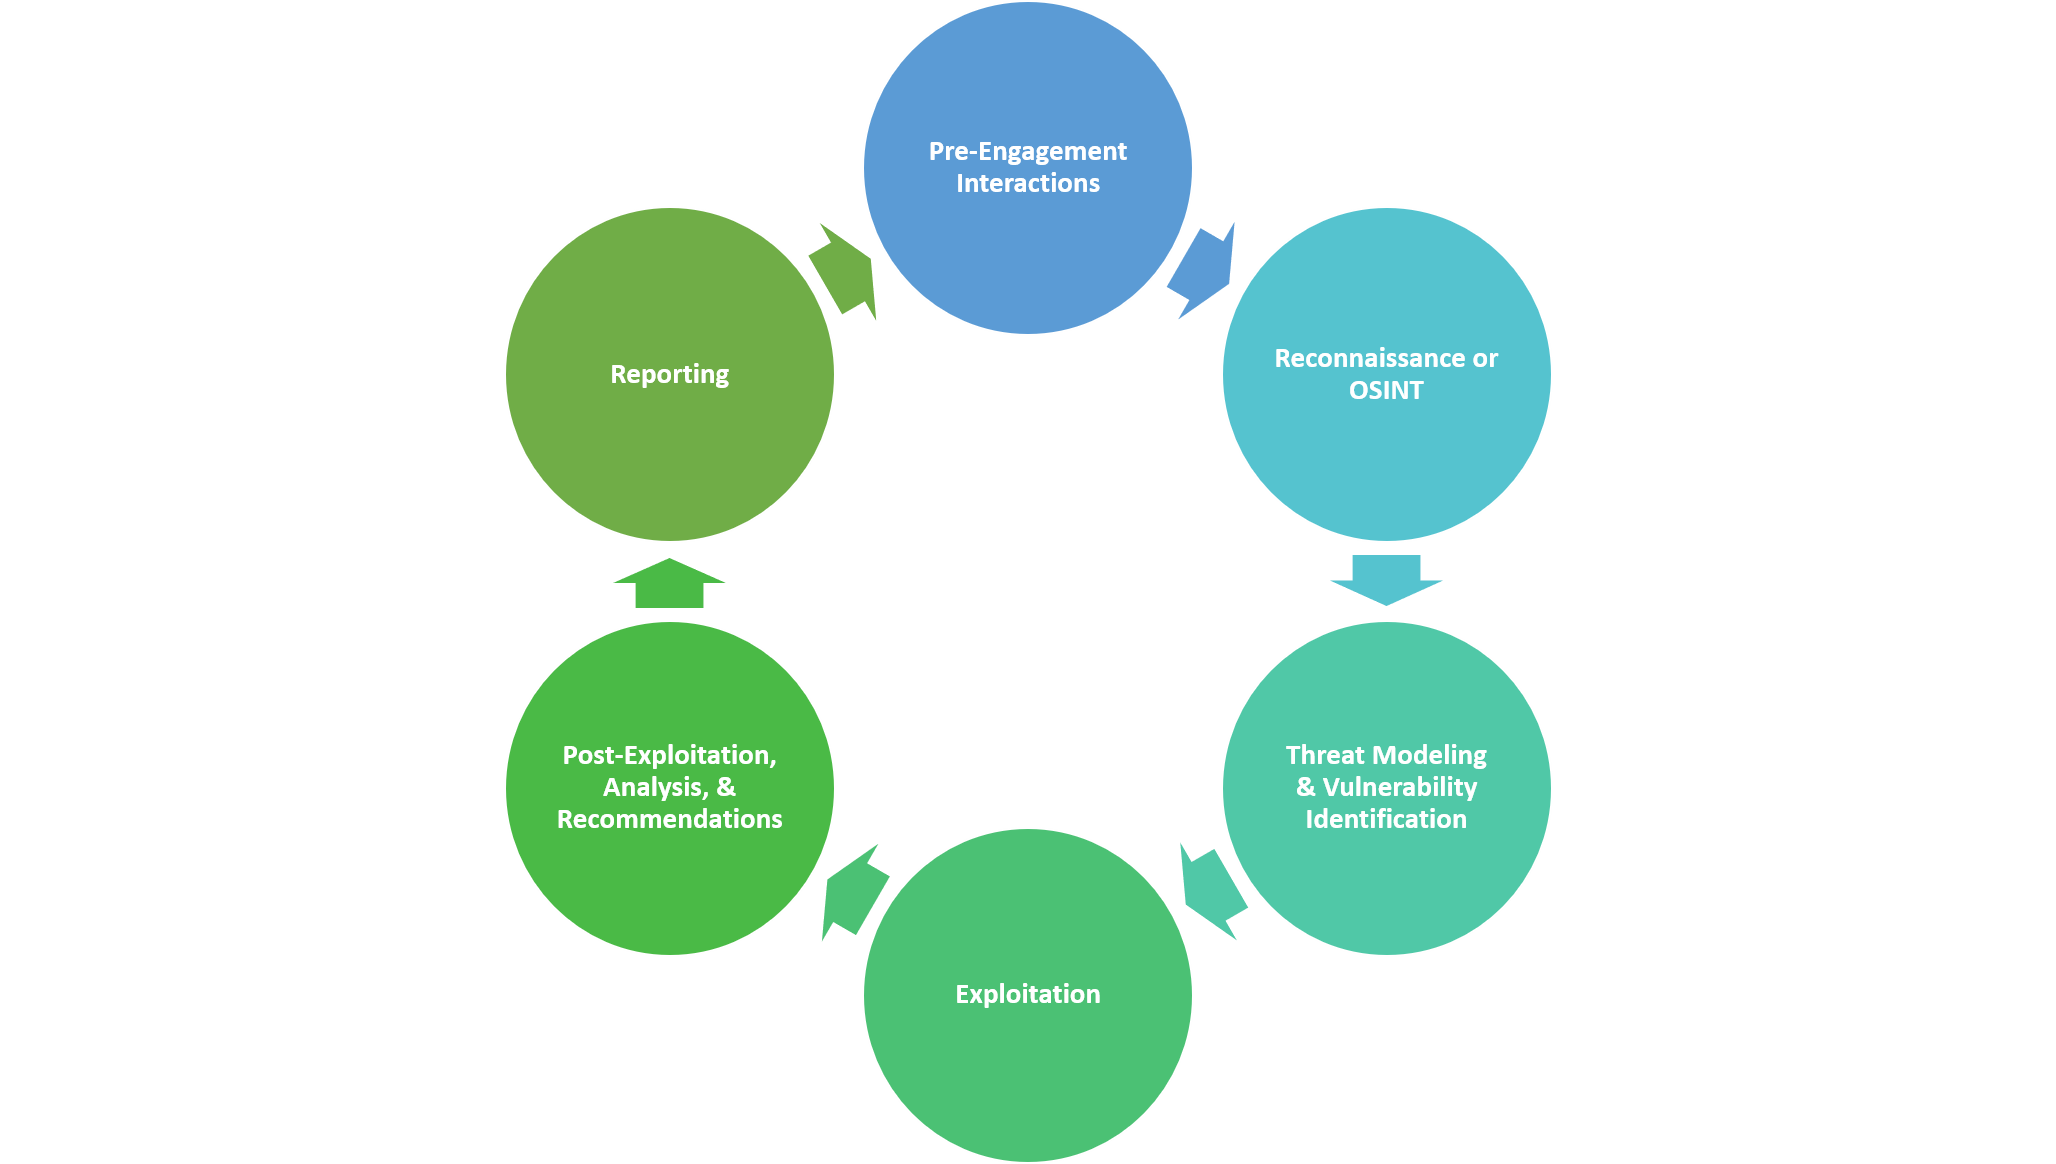
\includegraphics[width=\textwidth]{../drawable/decorations/penetration-testing-stages.png}
	\end{figure}

\end{frame}

% (6)
\definecolor{grin}{HTML}{5b9bd5}
\begin{frame}
	\frametitle{Pre-engagement interactions}
	
	\begin{columns}
		\column{0.66\linewidth}
		\onslide<1->{
		Penetration testing should start with \textit{pre-engagement} or \textit{scoping}:
	    }

	    \medskip

        \begin{itemize}
    		\item<2-> Expectations, targets, and goals of the test
    		\item<3-> Tools and frameworks used in the process
    		\item<4-> Legal implications, NDAs, risk evaluation, backup and emergency plans
    		\item<5-> \textbf{Black}, \textbf{grey} or \textbf{white} box testing types
    	\end{itemize}
    
    	\medskip
    
    	\onslide<6->{
    		Careful planning in these area is key for both the service owner and the pentester in order to deliver a thorough and accurate report.
	    }
		\column{0.33\linewidth}
		\centering
		\roundpic{0.9\textwidth}{0.9\textwidth}{../drawable/decorations/image-cloud-social.png}
	\end{columns}

\end{frame}

% (7)
\definecolor{grin}{HTML}{55C3CF}
\begin{frame}
	\frametitle{Reconnaissance}

	\onslide<1->{
		Next, intelligence is gathered through various methods, depending on the type of pentest agreed on. Usually, this revolves around:
	}

	\medskip

	\begin{itemize}
		\item<2-> \textbf{WHOIS} and \textbf{DNS} lookups
		\item<3-> \textbf{External footprinting} (search engine queries, social networks, etc...)
		\item<4-> \textbf{Internal footprinting} (port scanning, packet sniffing, OS fingerprinting, tailgating, etc...)
	\end{itemize}

	\medskip

	\onslide<5->{
		Pentesters are expected to gather as much information as possible in this phase in order to narrow down their effort in the following phase. For rounding out, the \textit{OSINT Framework} provides a thorough list of open information sources.
	}
\end{frame}

% (8)
\definecolor{grin}{HTML}{50C8A7}
\begin{frame}
	\frametitle{Threat modeling and vulnerability identification}

	\onslide<1->{
		This phase is devoted to preparatory work before the actual exploiting begins. Pentesters should:
	}
	
    \begin{columns}
		\column{0.6\linewidth}
		\begin{itemize}
    		\item<2-> Choose high-valued assets to be targeted
    		\item<3-> Identify vulnerabilities in each asset
    		\item<4-> Enumerate possible threats (either \textit{internal} or \textit{external}) and verify that the vulnerability is exploitable
    		\item<5-> Build payloads and map attack vectors to each vulnerability
    	\end{itemize}
		\column{0.4\linewidth}
		\centering
		\roundpic{0.9\textwidth}{0.9\textwidth}{../drawable/decorations/image-threat.jpg}
	\end{columns}

	\medskip

	\onslide<6->{
		At the end of this phase, a preliminary report on vulnerabilities is usually shared with the customer.
	}
\end{frame}

% (9)
\definecolor{grin}{HTML}{4BC174}
\begin{frame}
	\frametitle{Exploitation}

	\onslide<1->{
		This is the phase in which pentesters get their hands dirty. The objective is to see how far an attacker would be able to go when penetrating the network while avoiding detection and respecting the constraints agreed with the customer.
	}

	\medskip

	\onslide<2->{
		This is the phase in which Metasploit will be used in its fullest, although the framework provides assistance in all phases of pentesting.
	}

	\medskip

	\onslide<3->{
		The results of this phase will be the largest part of the report, for example:
		\begin{itemize}
			\item<4-> vulnerabilities, payloads, compromised machines
			\item<5-> time spent in the process
			\item<6-> hypothetical profit for the attacker
		\end{itemize}
	}

\end{frame}

% (10)
\definecolor{grin}{HTML}{4ABA46}
\begin{frame}
	\frametitle{Post-exploitation}

    \begin{columns}
		\column{0.3\linewidth}
		\centering
		
\includegraphics[width=\textwidth]{../drawable/decorations/image-checklist-whitebg.jpg}
		\column{0.7\linewidth}
		\onslide<1->{
		    Once a system has been compromised, several paths can be followed:
	    }

    	\begin{itemize}
    		\item<2-> attempting further access to \\ internal networks
    		\item<3-> setting up backdoors for future access
    		\item<4-> cleaning up logs and traces
    	\end{itemize}
	\end{columns}

	\medskip

	\onslide<5->{
		Post-exploitation, in general, refers to the steps taken after a successful exploits, in which pentesters are also expected to fully restore compromised systems to their clean state.
	}
\end{frame}

% (11)
\definecolor{grin}{HTML}{70AD47}
\begin{frame}
	\frametitle{Reporting}

	\onslide<1->{
		Finally, a written recommendation is produced from the pentester for the customer. The findings and explanations from the report will be used as guidelines for the customer' security posture and for future tests.
	}

	\centering
	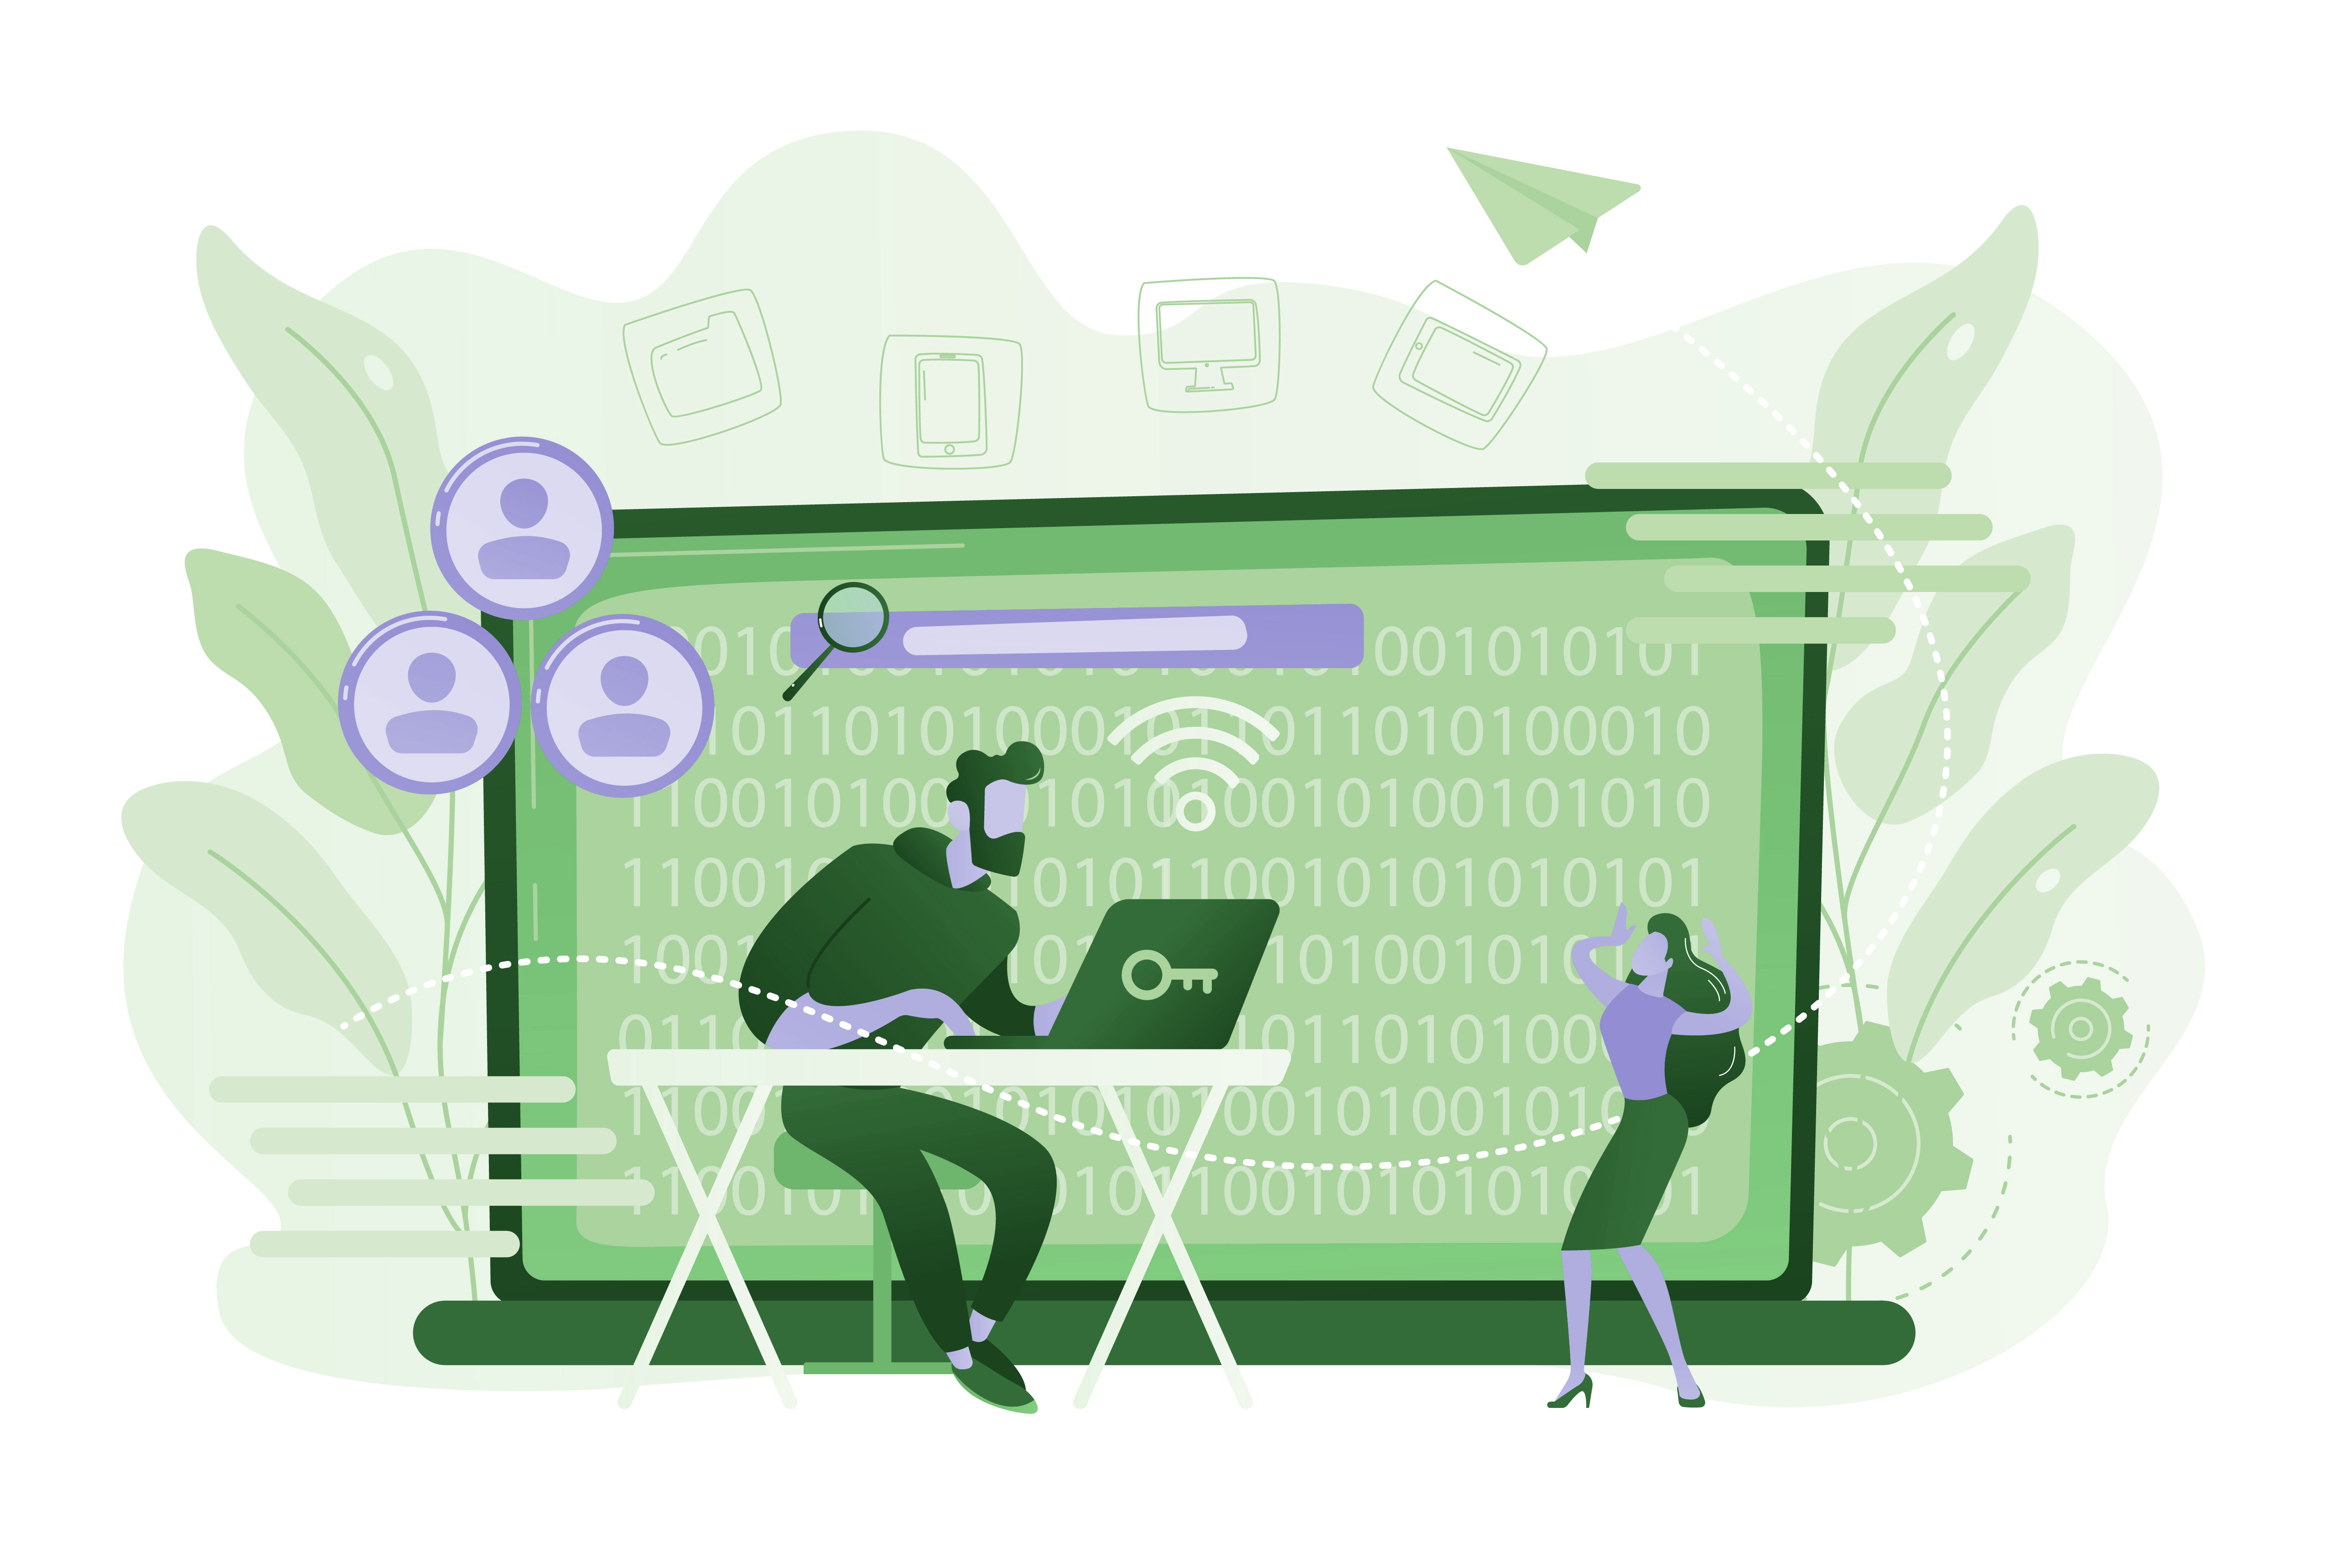
\includegraphics[width=0.65\textwidth]{../drawable/decorations/image-exploit-altcolor.jpg}
\end{frame}

% (12)
\definecolor{grin}{HTML}{0D78B9}
\section{Metasploit}

% (13)
\begin{frame}
	\frametitle{Metasploit}

	\begin{figure}[h]
		\centering
		
\includegraphics[width=.25\textwidth]{../drawable/logos/metasploit-logo.png}
	\end{figure}

	\begin{itemize}
		\item<2-> first released by H.D. Moore in 2003 with 11 exploits
		\item<3-> first written in Perl, later ported to Ruby
		\item<4-> de facto framework for exploit development
		\item<5-> used by attackers and pentesters alike
		\item<6-> as of 2021 bundled with over 2100 exploits and over 590 payloads
	\end{itemize}
\end{frame}

% (14)
\begin{frame}
	\frametitle{Cool, but...}

	\onslide<1->{
		what can we exactly do with Metasploit?
		\medskip
	}

	\begin{itemize}
		\item<2-> perform every phase from information gathering to exploiting and post-exploiting with automated tools, completion, and more
		\item<3-> use vendor-provided payloads and exploits - depending on the need, they can be mixed and matched - or write ones either from scratch or starting from known ones
		\item<4-> switch between CLI (\texttt{msfconsole}) and GUIs (\textit{web interface} or \textit{Armitage})
		\item<5-> use additional tools, such as Metasploitable, a vulnerable dummy machine ready to be tested
	\end{itemize}
\end{frame}

% (15)
\begin{frame}
	\frametitle{Modules}

	\begin{columns}
		\column{0.6\linewidth}

		\onslide<1->{
			Any task that can be performed in Metasploit is done with \textbf{modules}. Each one can perform a specific action, such as scanning or exploiting.
			\medskip
		}

		\onslide<2->{
			There are several types of modules available:
		}

		\begin{itemize}
			\item<3-> \textbf{Exploit} - an exploit is a sequence of commands to target a specific vulnerability found in a system or application (e.g. buffer overflow, code injection, etc...)
			\item<4-> \textbf{Auxiliary} - performs arbitrary actions, for example port scanning or DoS
		\end{itemize}

		\column{0.4\linewidth}
		\centering
		\includegraphics[width=\textwidth]{../drawable/decorations/image-cartoon-hacker.eps}
	\end{columns}

\end{frame}

% (16)
\begin{frame}
	\frametitle{Modules (cont.)}

	\begin{itemize}
		\item<1-> \textbf{Post-Exploitation} - assists in the homonymous phase by allowing data dumping, service enumeration, and more;
		\item<2-> \textbf{Payload} - the malicious shell code that runs after an exploit successfully compromises a system. Defines how you connect to the system, what to do, and more. Further sub-divided into \textbf{singles}, \textbf{stagers} and \textbf{stages}
		\item<3-> \textbf{NOP generator} - produces a series of random bytes that you can use to bypass standard IDS NOP sled signature and to pad buffers
	\end{itemize}

\end{frame}

% (17)
\begin{frame}[fragile]
	\frametitle{Commands}

	\begin{columns}
		\column{0.66\linewidth}
		This laboratory will focus on the basic usage of \texttt{msfconsole}, although all the exercises can be easily carried out on any interface.
		\begin{lstlisting}
help

search eternalblue

info 5
        \end{lstlisting}
		\column{0.33\linewidth}
		\centering
		\roundpic{0.9\textwidth}{0.9\textwidth}{../drawable/decorations/image-eternalblue.jpg}
	\end{columns}

\end{frame}

% (18)
\begin{frame}[fragile]
	\frametitle{Commands}

	\begin{columns}
		\column{0.66\linewidth}
		This laboratory will focus on the basic usage of \texttt{msfconsole}, although all the exercises can be easily carried out on any interface.
		\begin{lstlisting}
help

search platform:windows \
    description:acrobat

info 14
        \end{lstlisting}
		\column{0.33\linewidth}
		\centering
		
\includegraphics[width=0.9\textwidth]{../drawable/decorations/image-acrobat.jpg}
	\end{columns}

\end{frame}

% (19)
\begin{frame}[fragile]
	\frametitle{Commands}

	\begin{columns}
		\column{0.66\linewidth}
		This laboratory will focus on the basic usage of \texttt{msfconsole}, although all the exercises can be easily carried out on any interface.
		\begin{lstlisting}
help

search cve:2021 type:exploit

info 1
        \end{lstlisting}
		\column{0.33\linewidth}
		\centering
		
\includegraphics[width=0.9\textwidth]{../drawable/decorations/image-cve.jpg}
	\end{columns}

\end{frame}

% (20)
\begin{frame}[fragile]

	\frametitle{Commands}

	\begin{columns}
		\column{0.4\linewidth}
		\centering
		\includegraphics[width=\textwidth]{../drawable/decorations/image-checklist-fromright.eps}
		\column{0.6\linewidth}
		Once an exploit has been chosen, we can fine tune it, starting from the possible payloads.
		\begin{lstlisting}
use 14

show payloads 
search type:payload 

set payload [...]
        \end{lstlisting}
	\end{columns}

\end{frame}

% (21)
\begin{frame}[fragile]

	\frametitle{Commands}

	\begin{columns}
		\column{0.6\linewidth}
		Options can be set and unset depending on needs.
		\begin{lstlisting}
show options

set FILENAME file.pdf
unset RPORT
        \end{lstlisting}
		\column{0.4\linewidth}
		\centering
		\roundpic{0.8\textwidth}{0.8\textwidth}{../drawable/decorations/image-pdfdownload.png}
	\end{columns}

\end{frame}

% (22)
\begin{frame}[fragile]

	\frametitle{Commands}

	\begin{columns}
		\column{0.5\linewidth}
		\centering
		\includegraphics[width=\textwidth]{../drawable/decorations/image-generic.eps}
		\column{0.5\linewidth}
		Finally, we can launch the exploit or just verify it with some simple commands:
		\begin{lstlisting}
check
exploit

back
        \end{lstlisting}
	\end{columns}
\end{frame}

% (23)
\begin{frame}[fragile]

	\frametitle{Commands}

	However, Metasploit isn't just for blindly throwing exploits at targets. In the framework we can find several tools that can aid in all phases of penetration testing, or provide further customizations to exploits. For example:

	\medskip

	\begin{lstlisting}
edit    grep    irb    jobs    kill     sessions
    \end{lstlisting}

	\medskip

	Let us now dive deeper into Metasploit and get our hands dirty.
	
	\begin{figure}
    	\centering
    	\includegraphics[width=0.45\textwidth]{../drawable/decorations/image-getstarted.eps}
	\end{figure}
	
\end{frame}

\definecolor{grin}{HTML}{22252E}

% (24)
\section{Exercises}

\subsection{Preliminaries}

% (25)
\begin{frame}
    \frametitle{Preliminaries}
    
    We start by examining the network at our disposal. 
    
    \begin{figure}
    	\centering
    	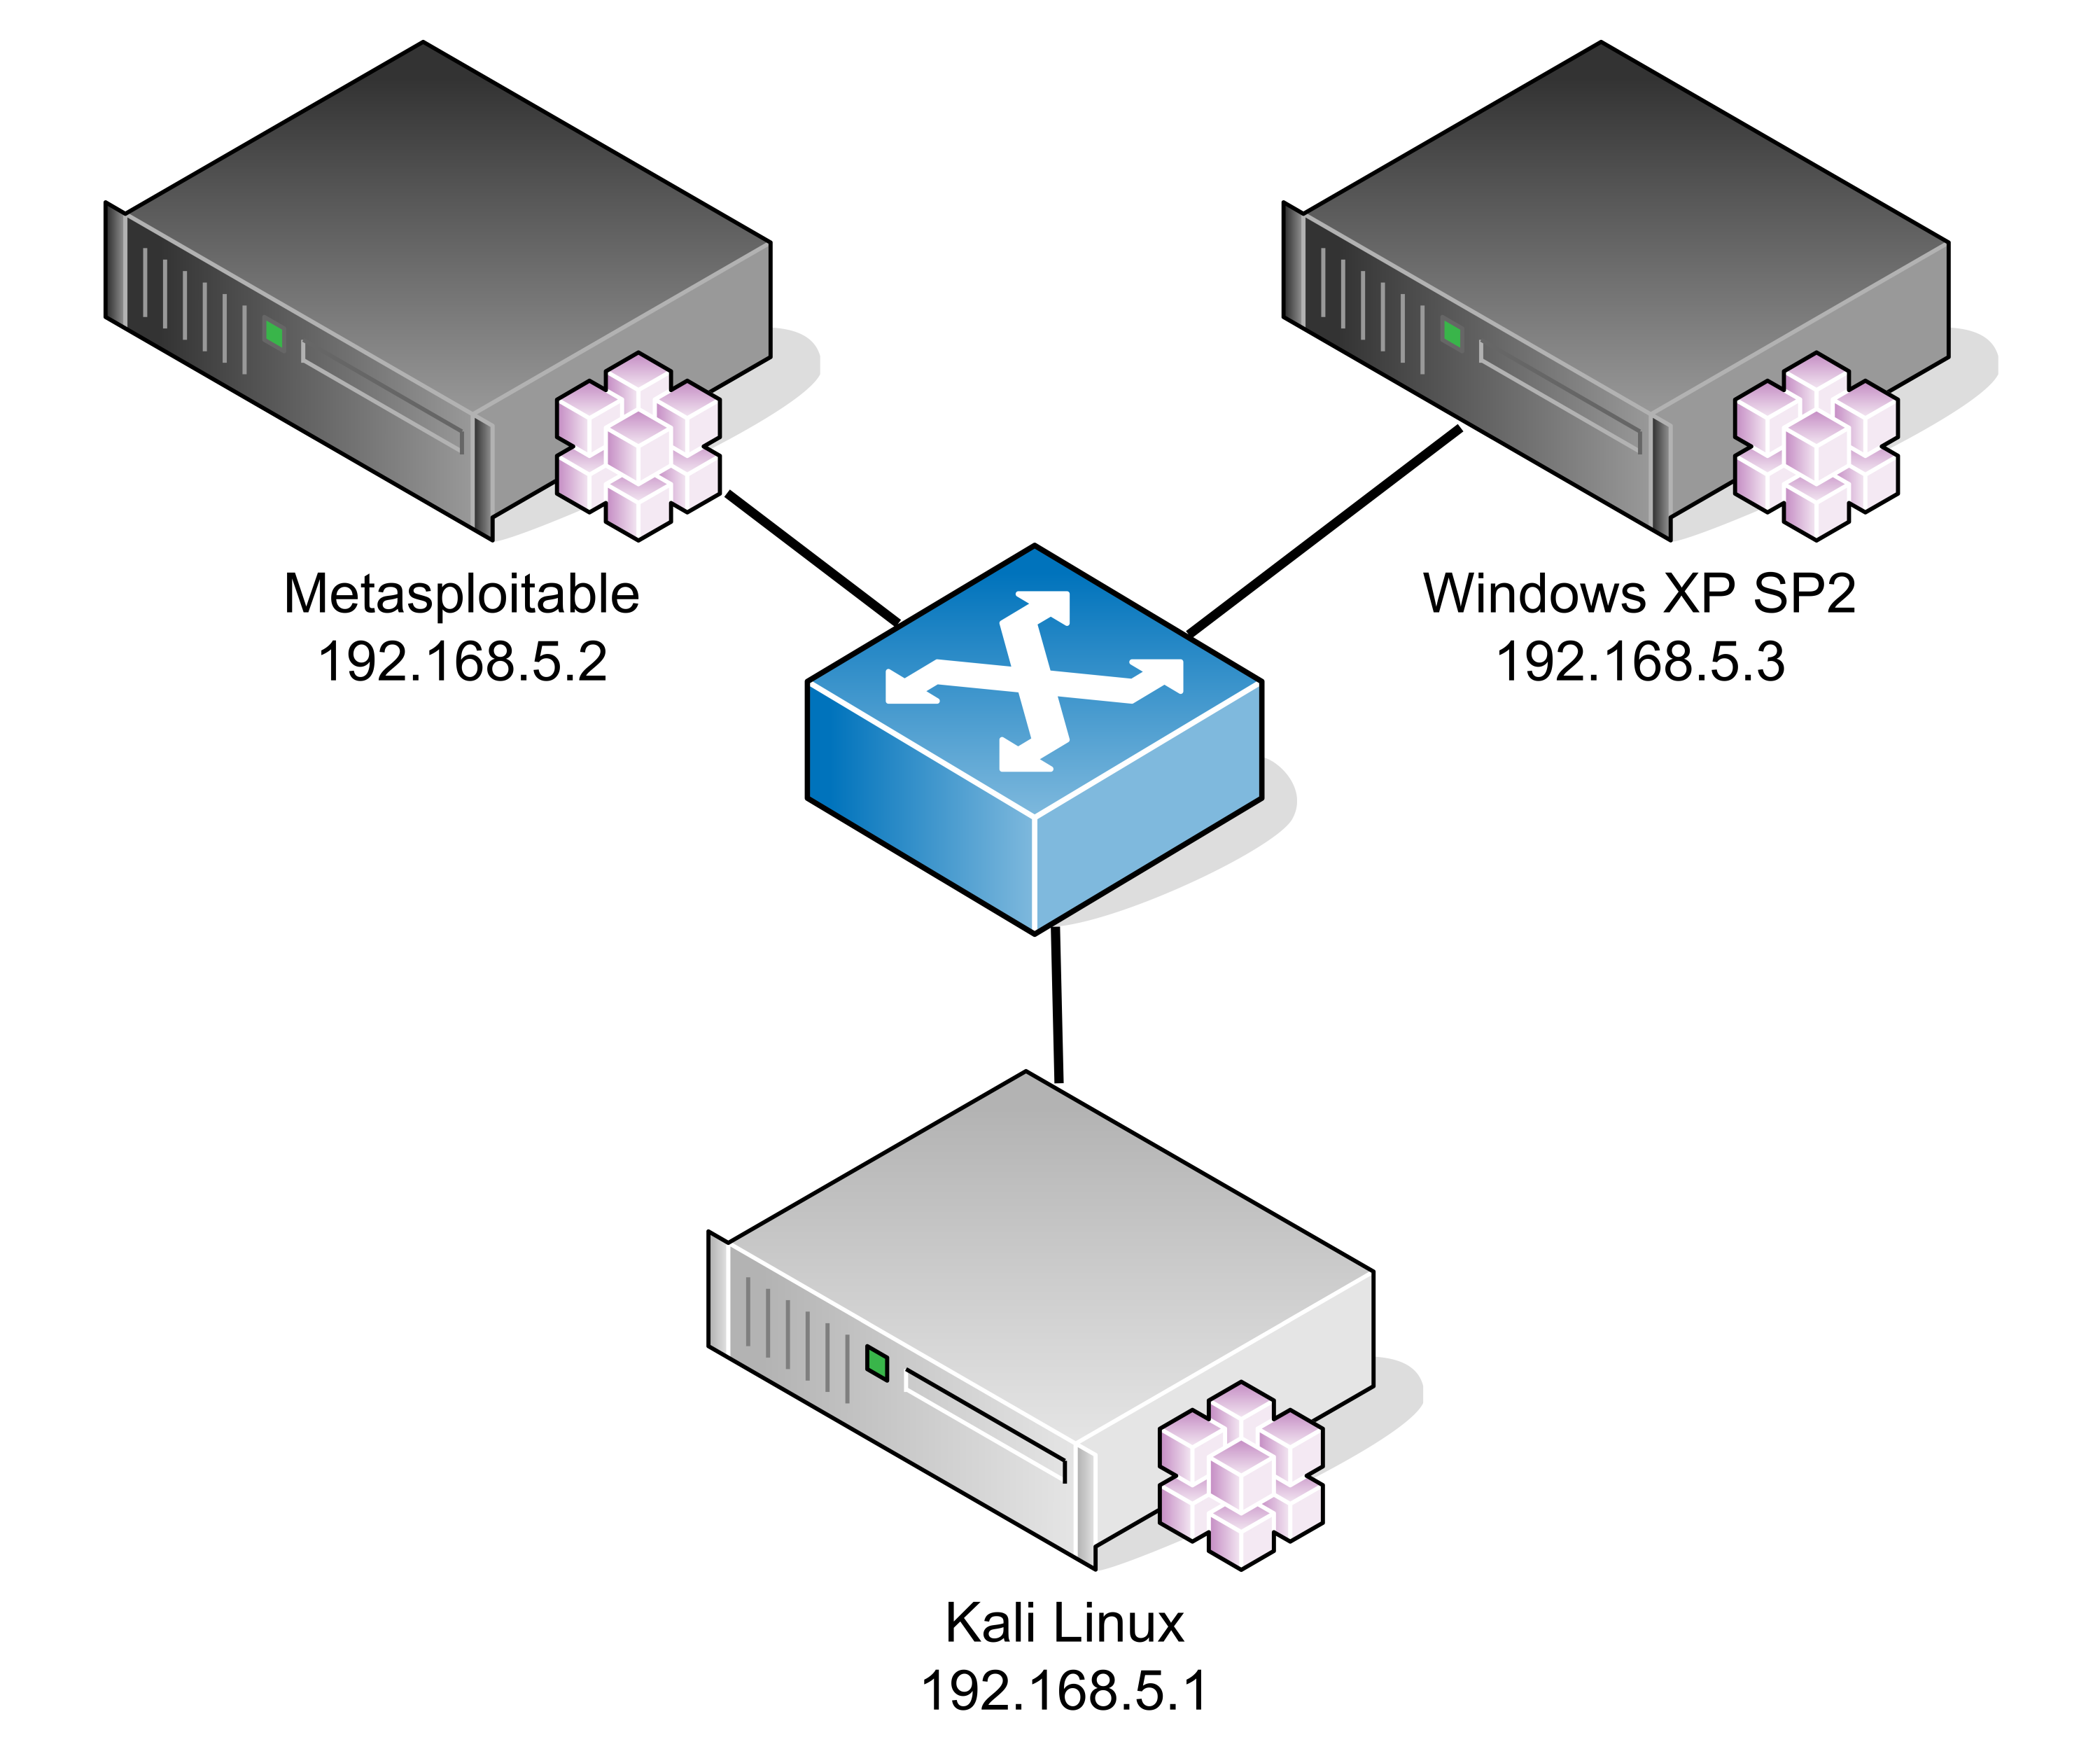
\includegraphics[width=0.6\textwidth]{../drawable/preliminaries_screenshots/prel-net.png}
	\end{figure}
\end{frame}

% (26)
\begin{frame}
    \frametitle{Preliminaries}
    
    To get started, we boot all three VMs and verify the three IPs on the \texttt{intnet} network.
    
	\begin{figure}
    	\centering
    	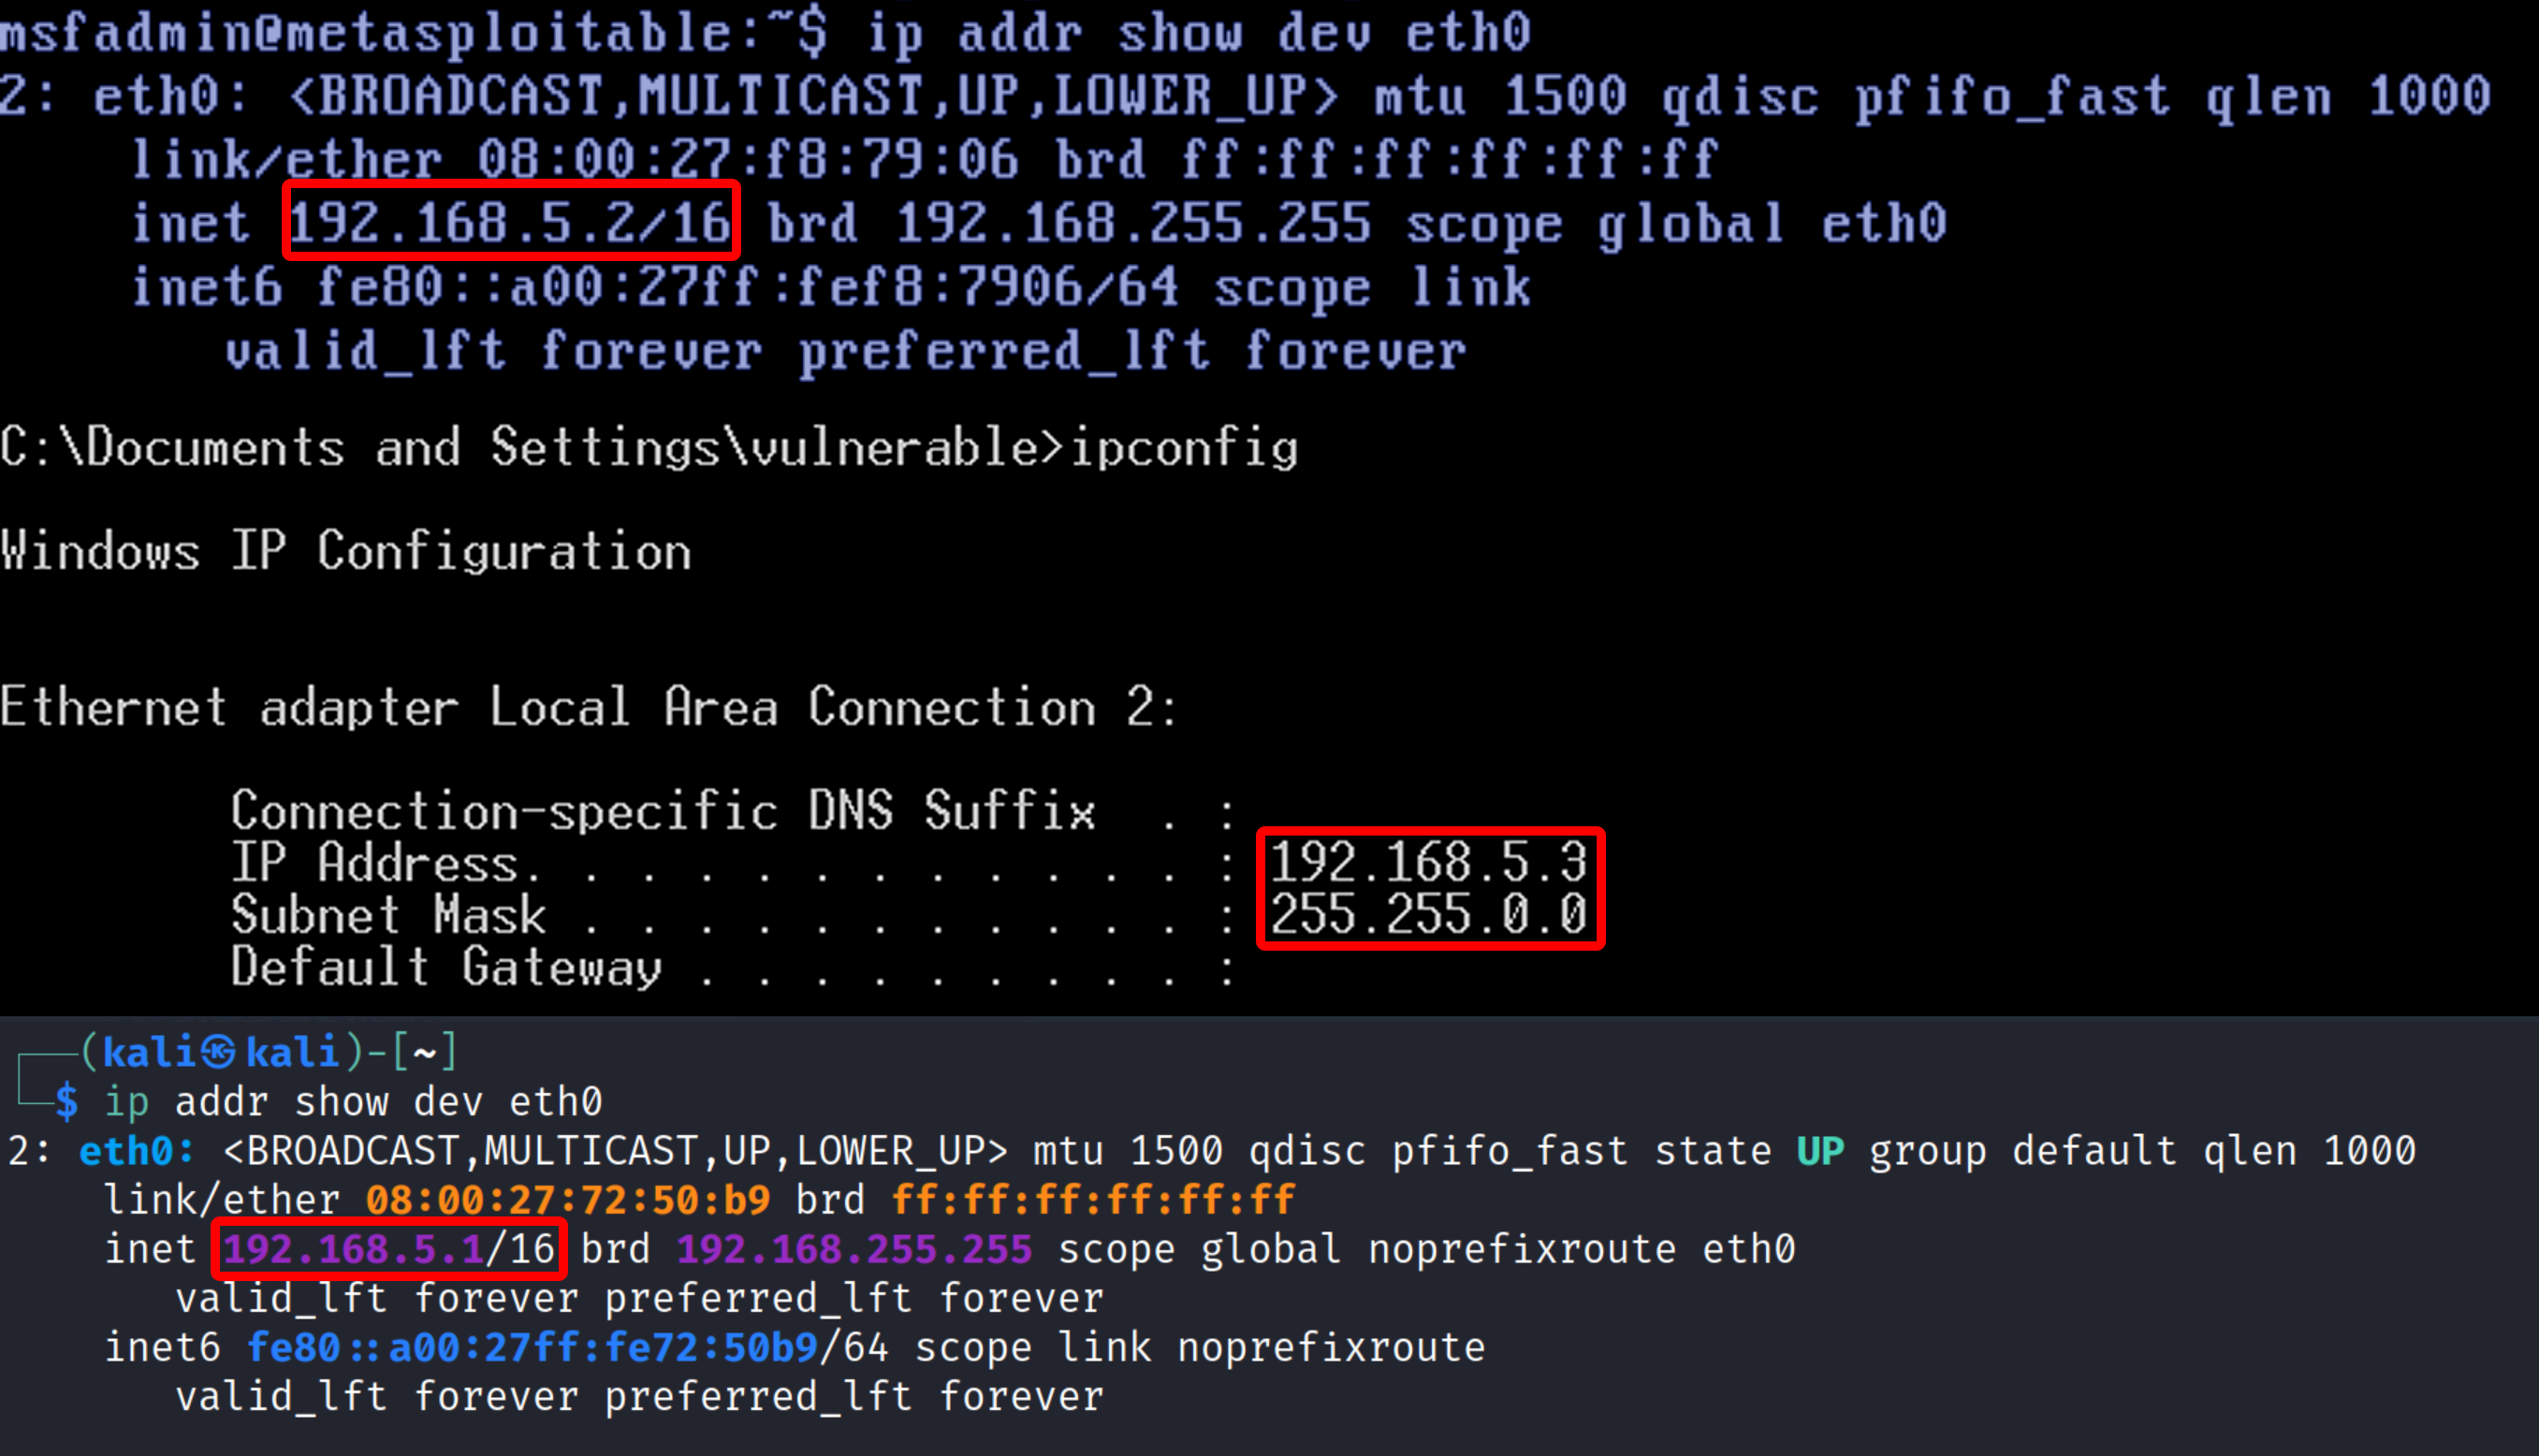
\includegraphics[width=0.9\textwidth]{../drawable/preliminaries_screenshots/prel-ips.png}
	\end{figure}
    
\end{frame}

% (27)
\begin{frame}
    \frametitle{Preliminaries}
    
    Then, we open a terminal on Kali and fire up \texttt{sudo msfconsole}:
	
	\begin{figure}
    	\centering
    	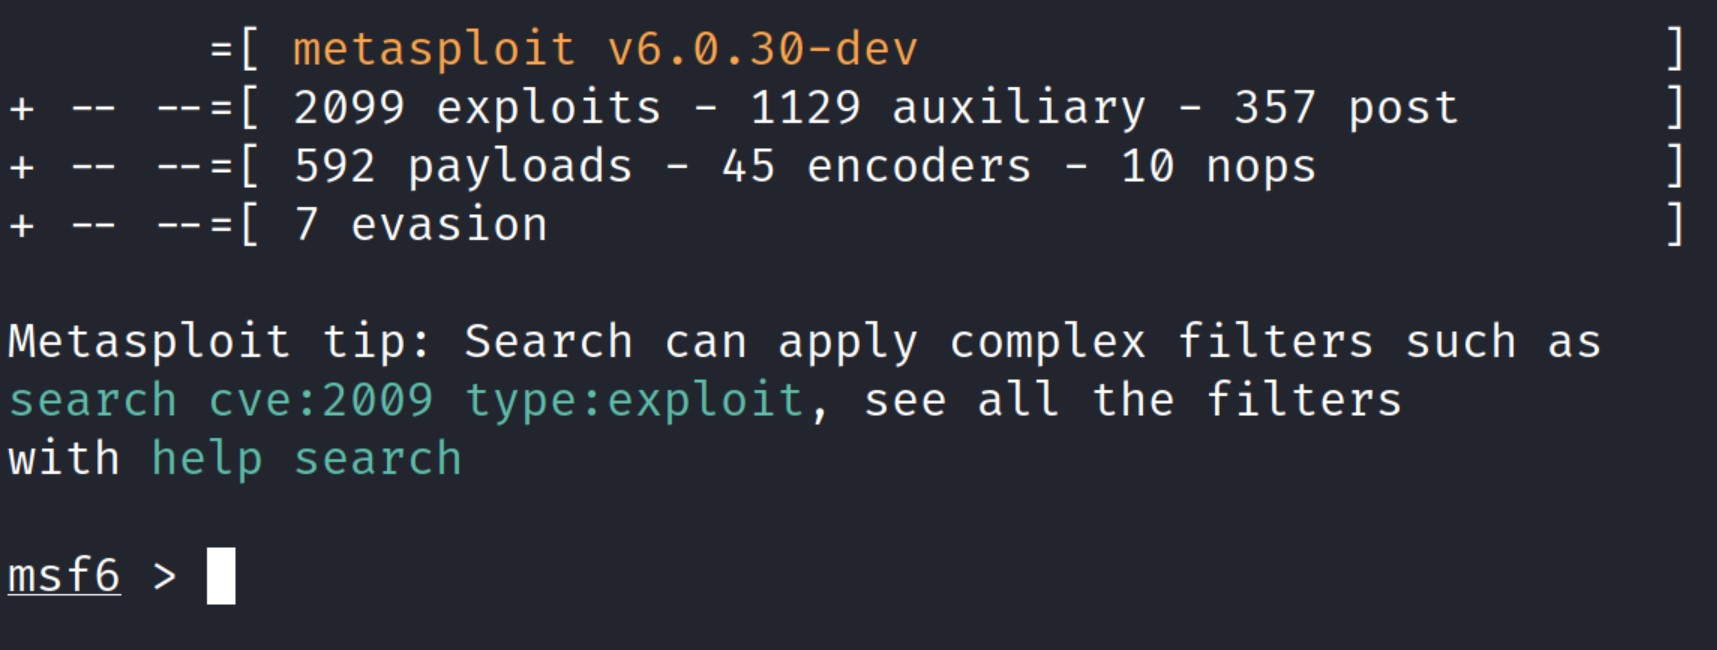
\includegraphics[width=0.9\textwidth]{../drawable/preliminaries_screenshots/prel-msfconsole.jpg}
    \end{figure}
\end{frame}

\subsection{Exercise 1}

% (28)
\begin{frame}
	\frametitle{Exercise 1: Reconnaissance}
	
	\frametitle{Commands}

	\begin{columns}
		\column{0.7\linewidth}	
		\onslide<1-> {
		First, we make use of Metasploit's deep auxiliary \textit{EXploitation} library, \texttt{lib/msf/core}, for automating typical reconnaissance tasks. It is completely written in Ruby.

		\medskip
	}

	\onslide<2-> {
		An auxiliary is simply a packaged exploit without a payload. The syntax requires the use of \texttt{run} instead of \texttt{exploit}.

		\medskip
	}

	\onslide<3-> {
		Components include scanners, fuzzers, DoS managers, but also sophisticated administrative access exploits such as brute forcers and directory traversal components.
	}
	\column{0.3\linewidth}
	\centering
		\roundpic{0.8\textwidth}{\textwidth}{../drawable/decorations/image-fingerprint.eps}
	\end{columns}
\end{frame}

% (29)
\begin{frame}
    \frametitle{Exercise 1: Reconnaissance}
    
    \onslide<1->{
        Let us start by examining open some ports on our targets. We can either use \textbf{Nmap} or one of the auxiliary Metasploit modules:
    }
    
	\begin{figure}
    	\centering
    	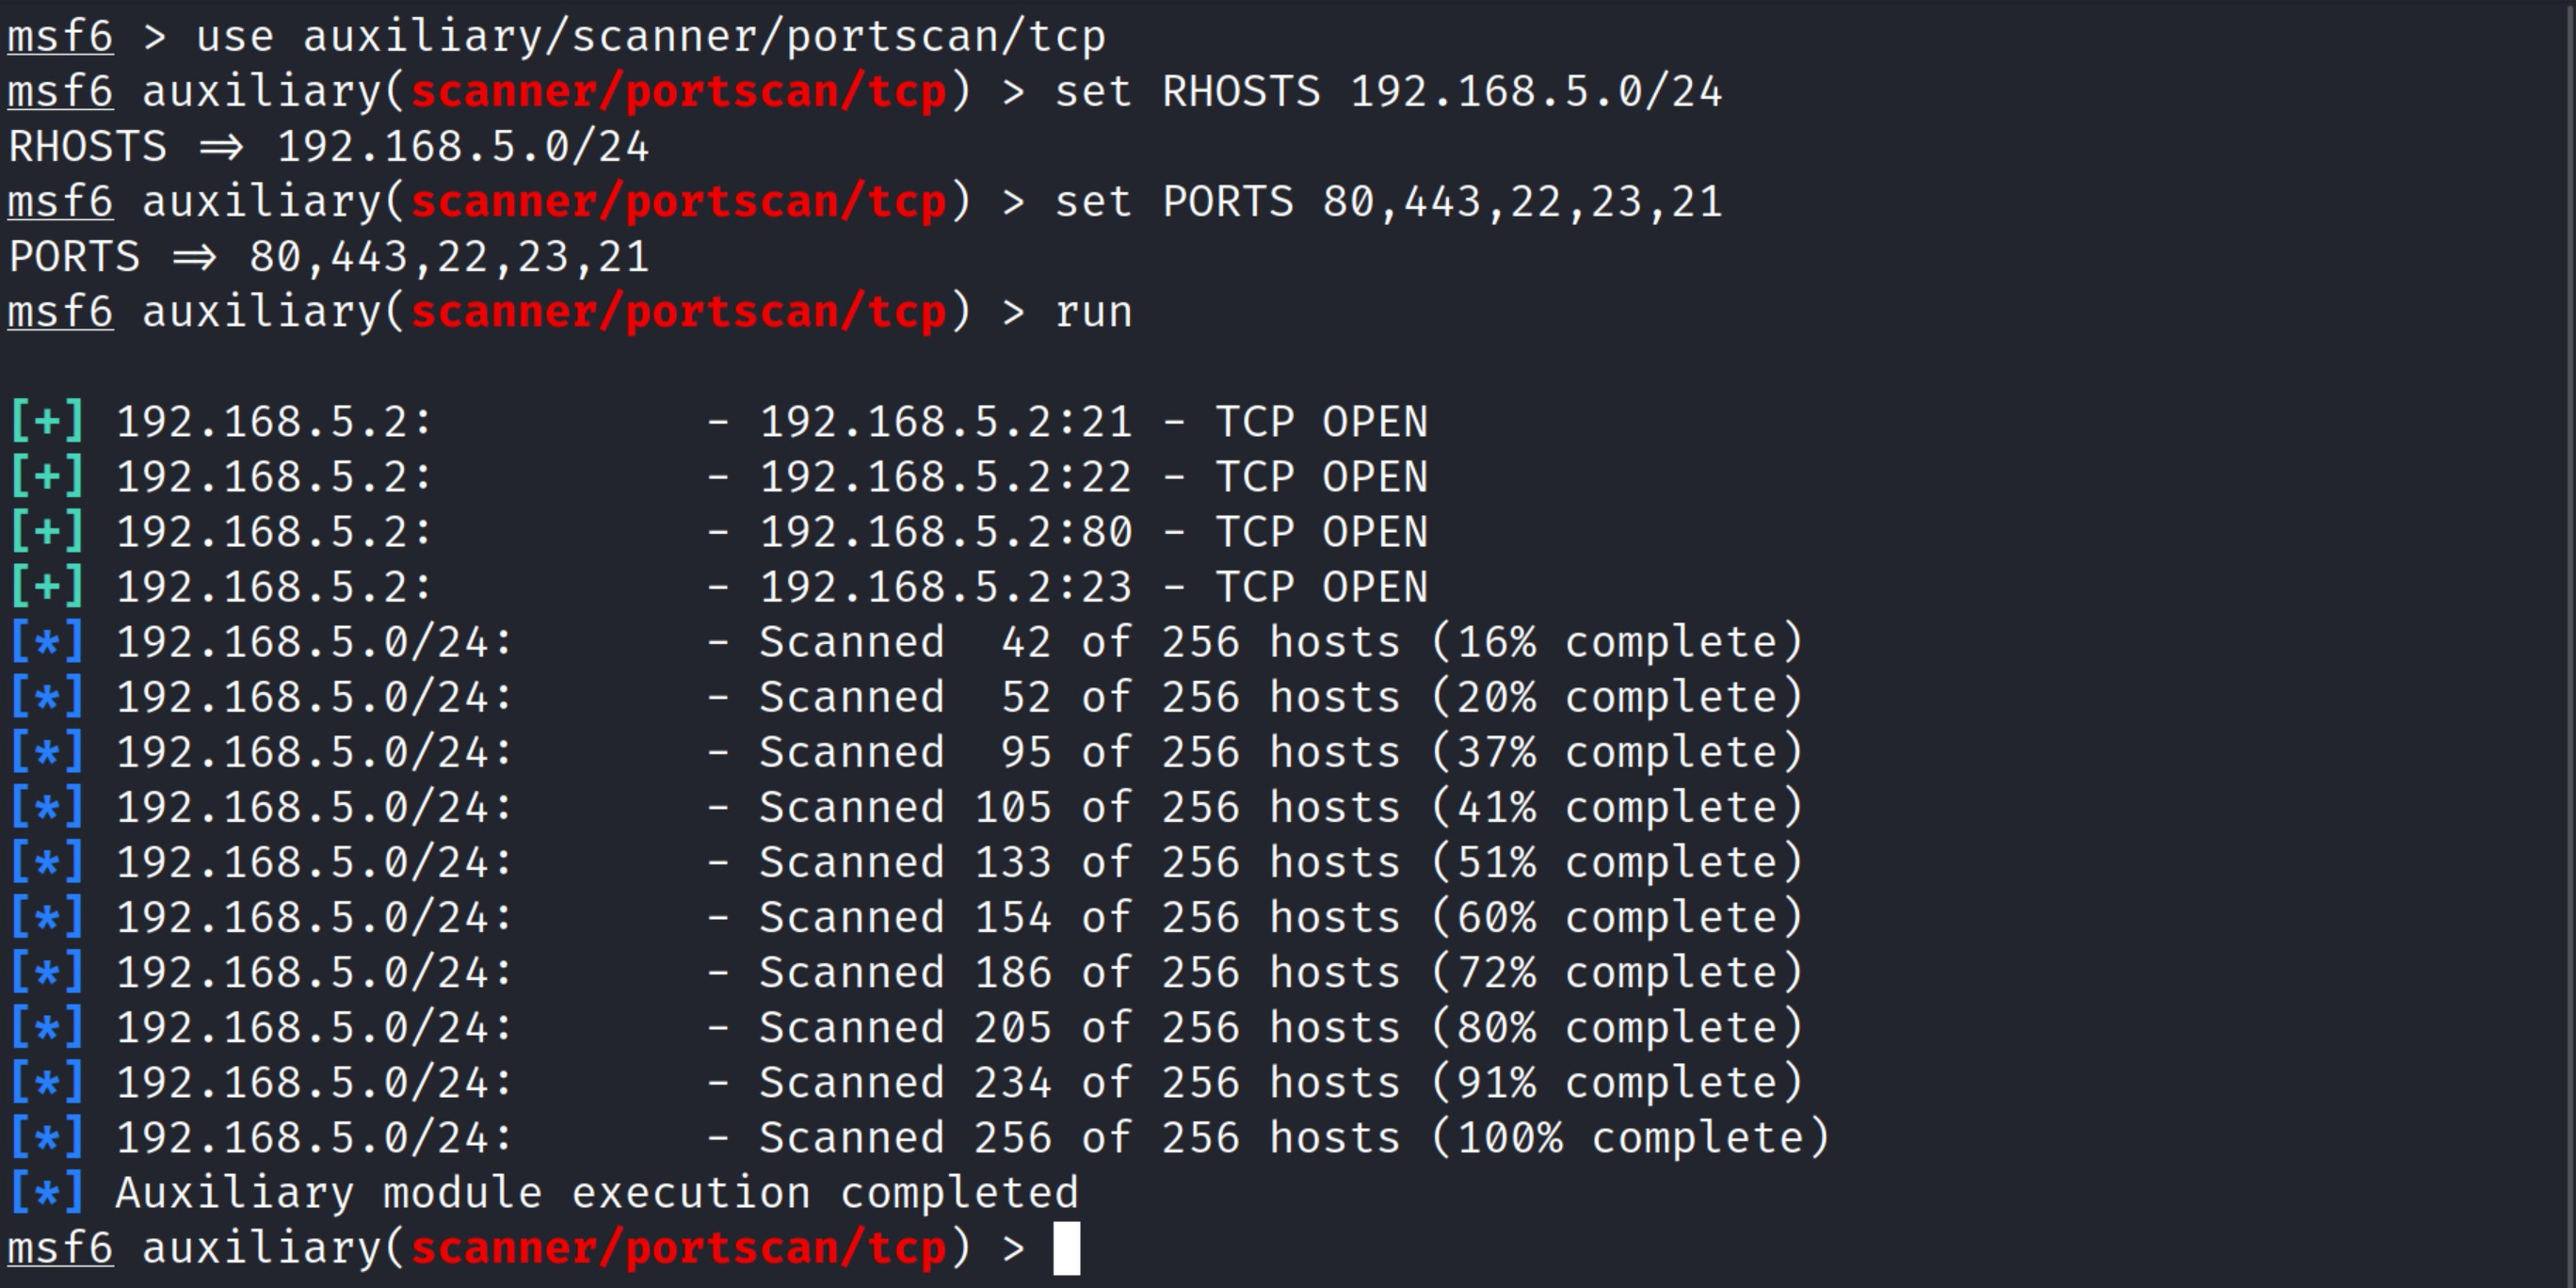
\includegraphics[width=0.8\textwidth]{../drawable/exercise_1_screenshots/es1-scan.jpg}
	\end{figure}
	
    \onslide<2->{
        For now, we will use a \texttt{TCP} scan. In the next exercise a more complete scan will be performed.
    }
    
	
\end{frame}

% (30)
\begin{frame}
    \frametitle{Exercise 1: Reconnaissance}
    Metasploit can provide further aid, for example by fingerprinting the \texttt{SSH} version:
    
	\begin{figure}
    	\centering
    	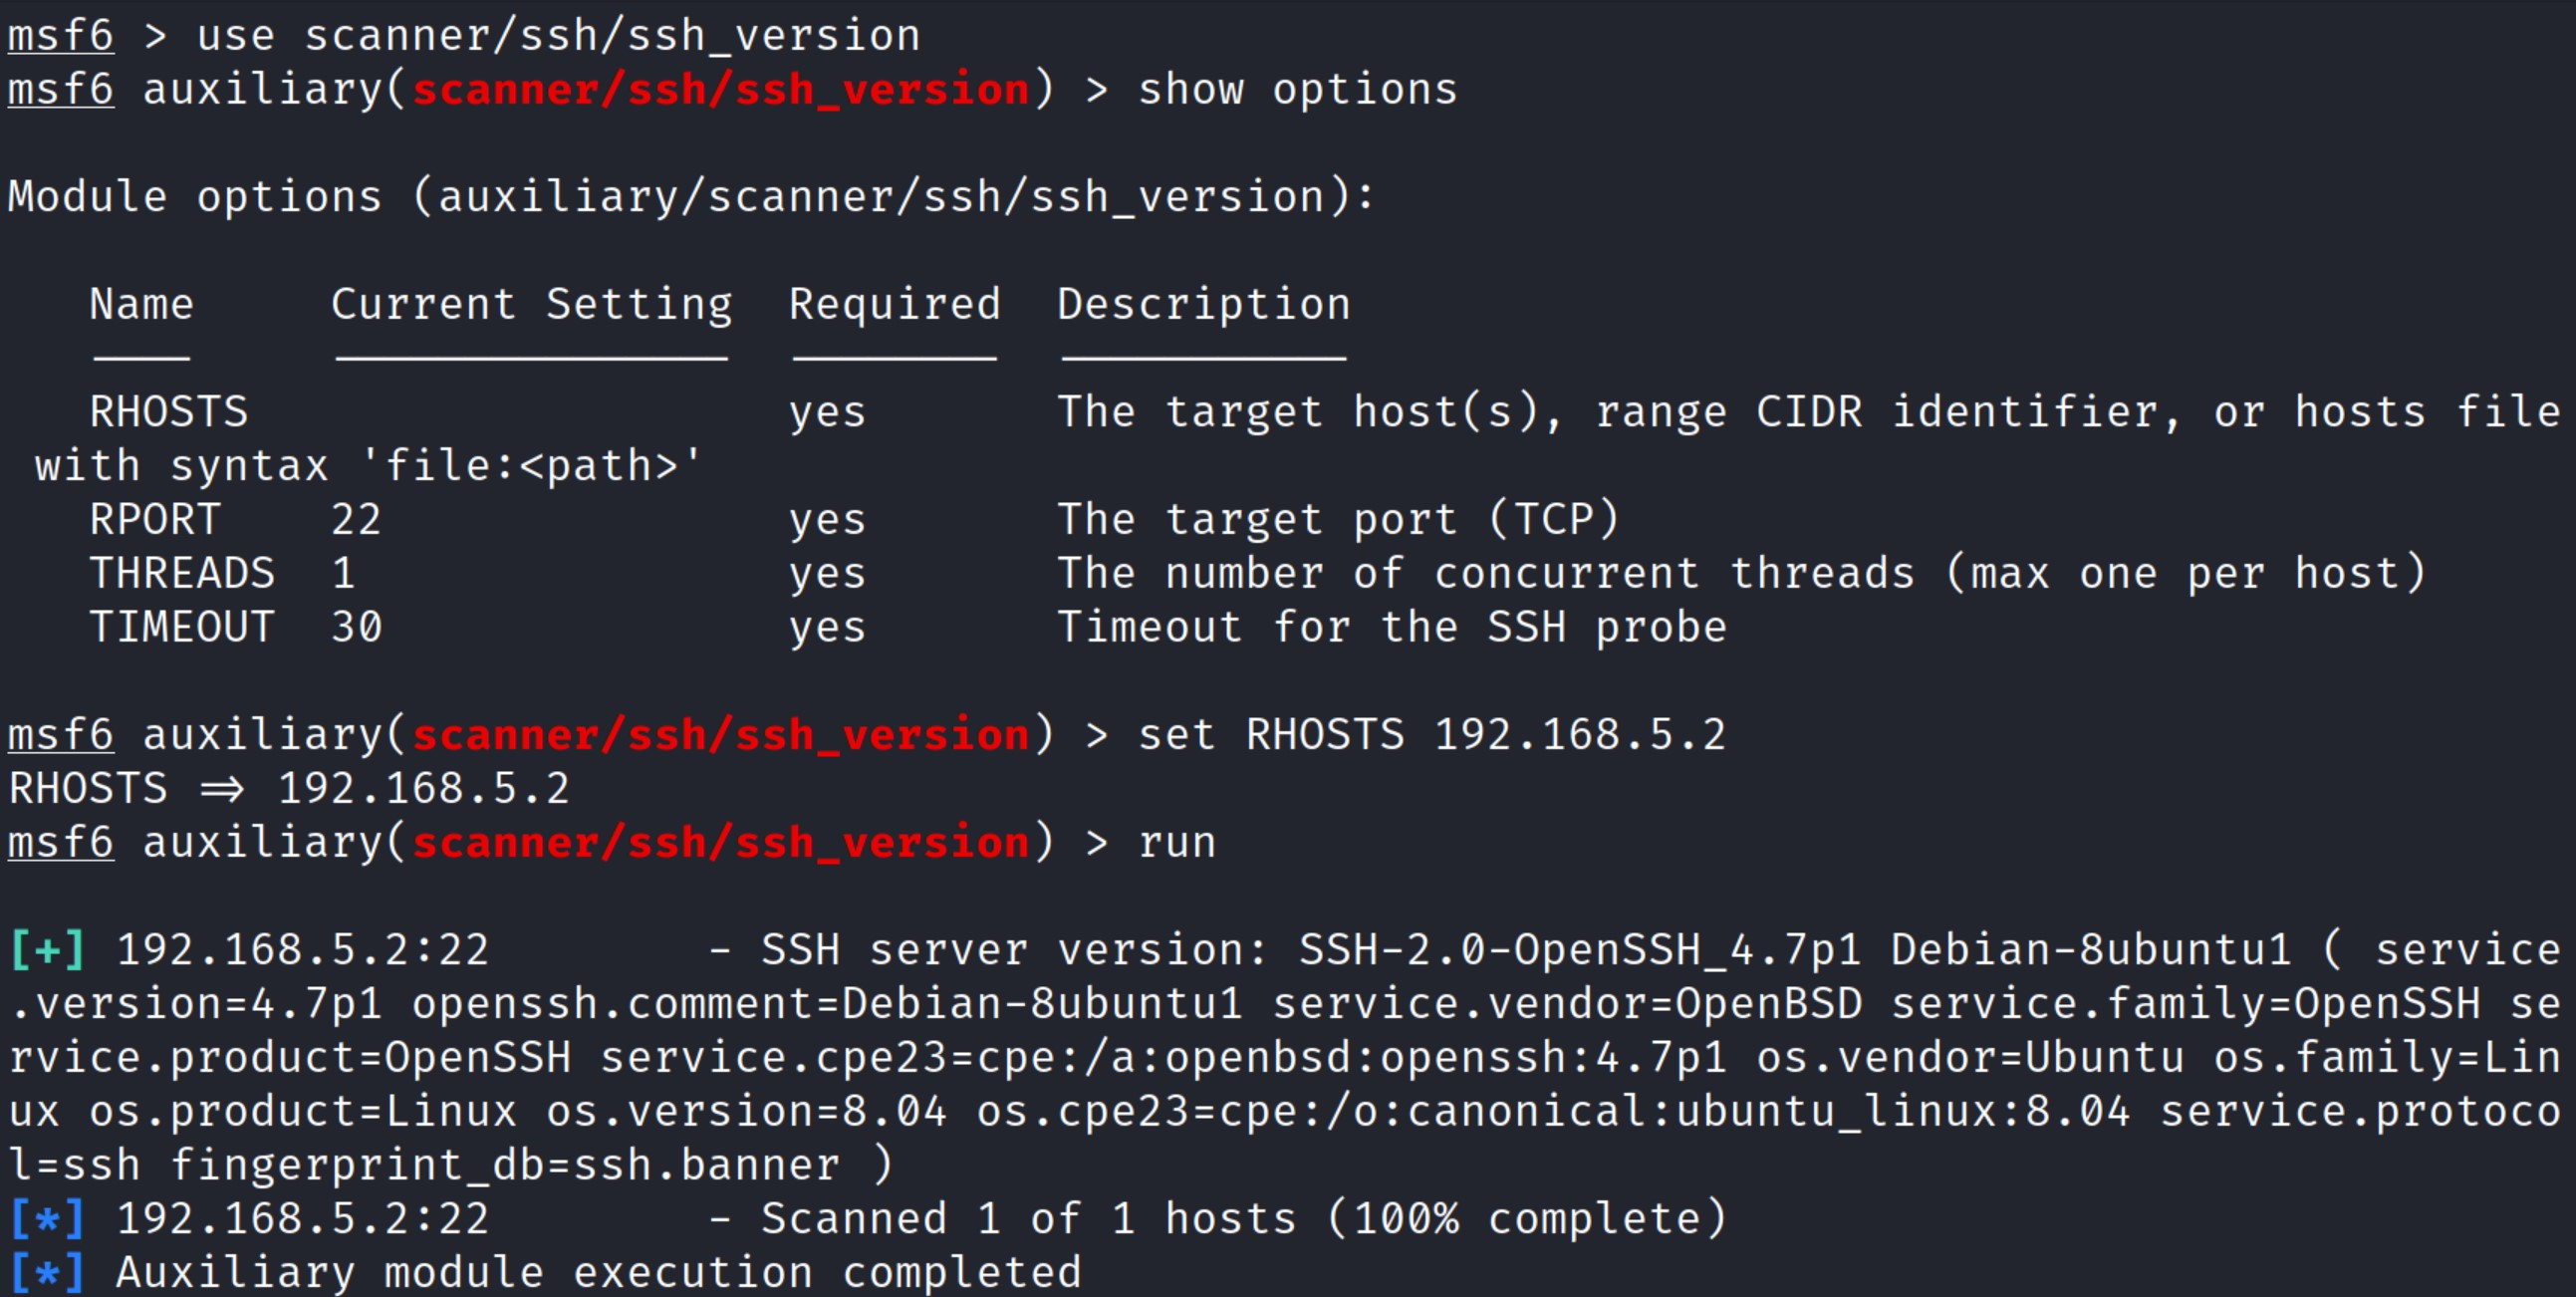
\includegraphics[width=0.9\textwidth]{../drawable/exercise_1_screenshots/es1-ssh.jpg}
	\end{figure}
\end{frame}

% (31)
\begin{frame}
    \frametitle{Exercise 1: Reconnaissance}
    As this is a regular OpenSSH server on Ubuntu 8, we can try to brute-force our way inside using the \texttt{ssh\_login} module.
    
	\begin{figure}
		\centering
		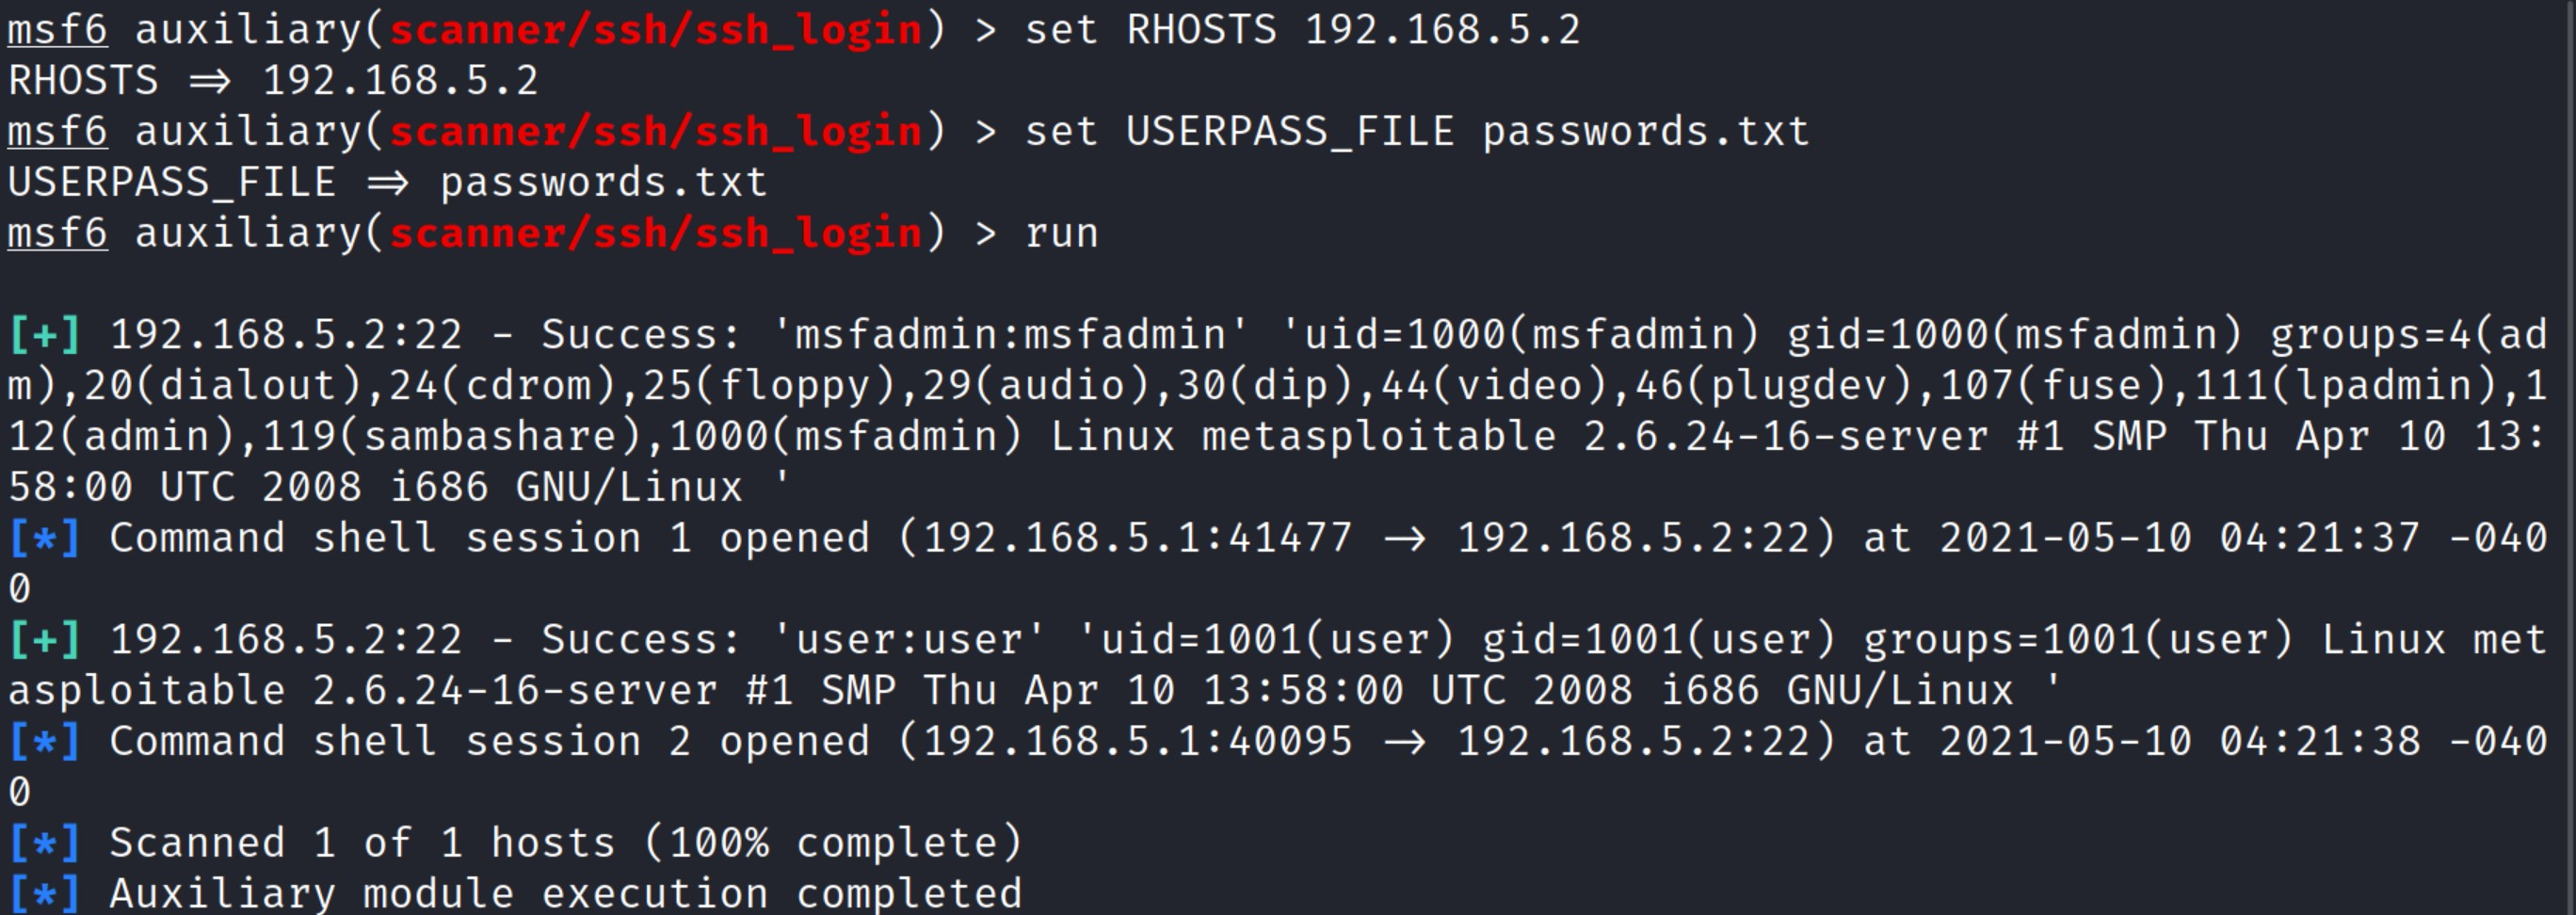
\includegraphics[width=\textwidth]{../drawable/exercise_1_screenshots/es1-brutessh.jpg}
	\end{figure}
\end{frame}

% (32)
\begin{frame}
    \frametitle{Exercise 1: Reconnaissance}
    
    \onslide<1->{    
        The provided file provided two valid username/password combinations. We can check the active sessions with the \texttt{sessions} command:
    }
    
	\begin{figure}
		\centering
		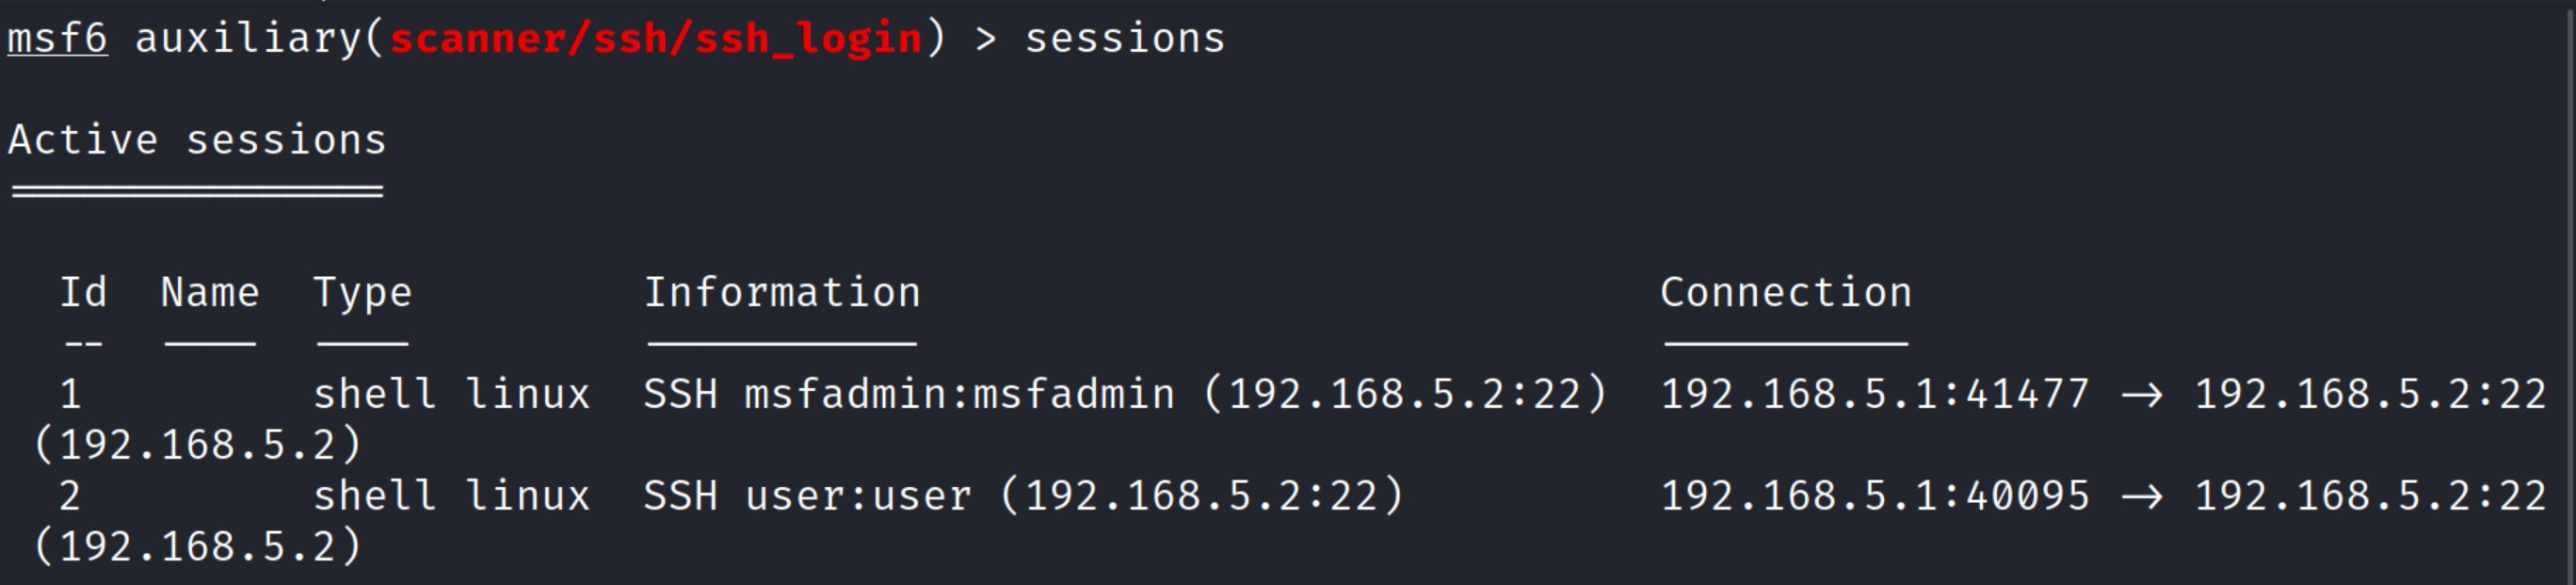
\includegraphics[width=\textwidth]{../drawable/exercise_1_screenshots/es1-sshsessions.jpg}
	\end{figure}
	
	\onslide<2->{
	    Notice the difference in privileges between the two shells. 
	}
\end{frame}

% (33)
\begin{frame}
    \frametitle{Exercise 1: Reconnaissance}
    The amount of modules is vast. For example, we can check the running version of a web server, or list its available directories:
    
	\begin{figure}
    	\centering
    	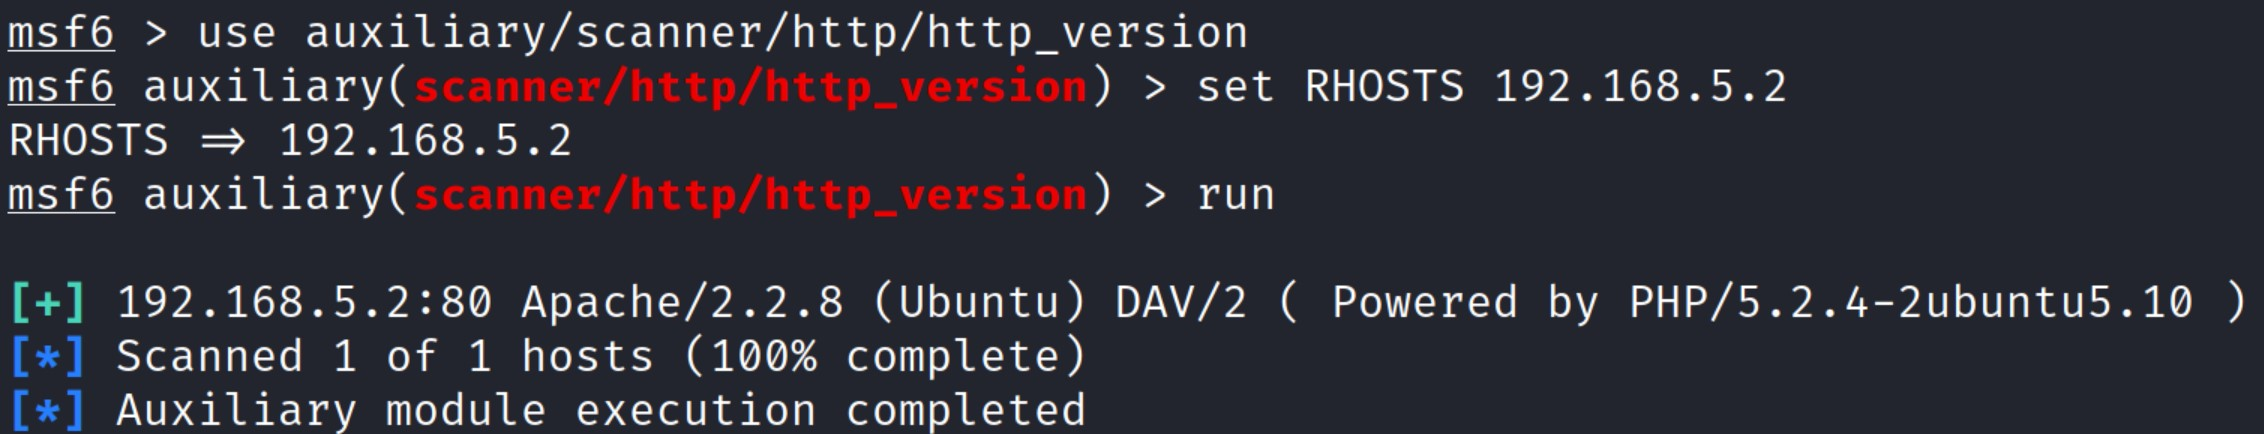
\includegraphics[width=0.9\textwidth]{../drawable/exercise_1_screenshots/es1-http.jpg}
    	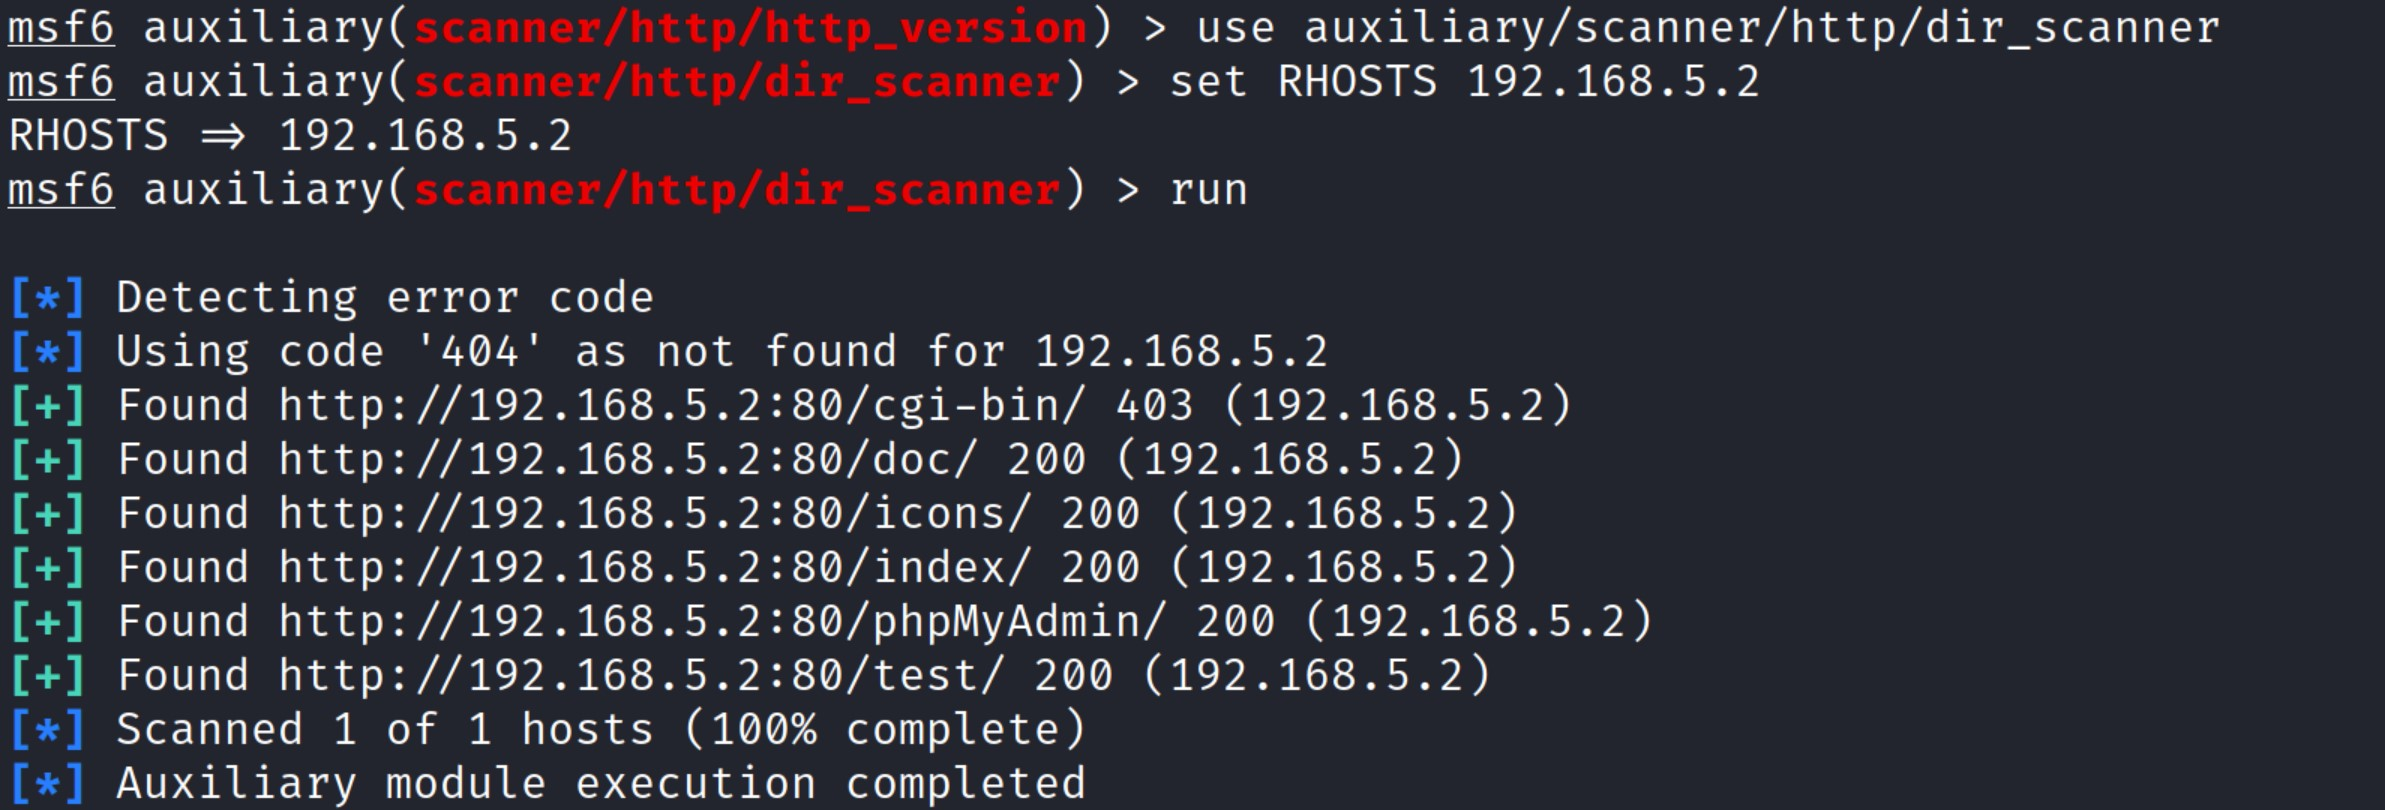
\includegraphics[width=0.9\textwidth]{../drawable/exercise_1_screenshots/es1-httpdir.jpg}
	\end{figure}
\end{frame}

% (34)
\begin{frame}
    \frametitle{Exercise 1: Reconnaissance}
    When scanning vast networks setting the \texttt{THREADS} variable can prove useful. Here is a real-world example.
    
	\begin{figure}
		\centering
		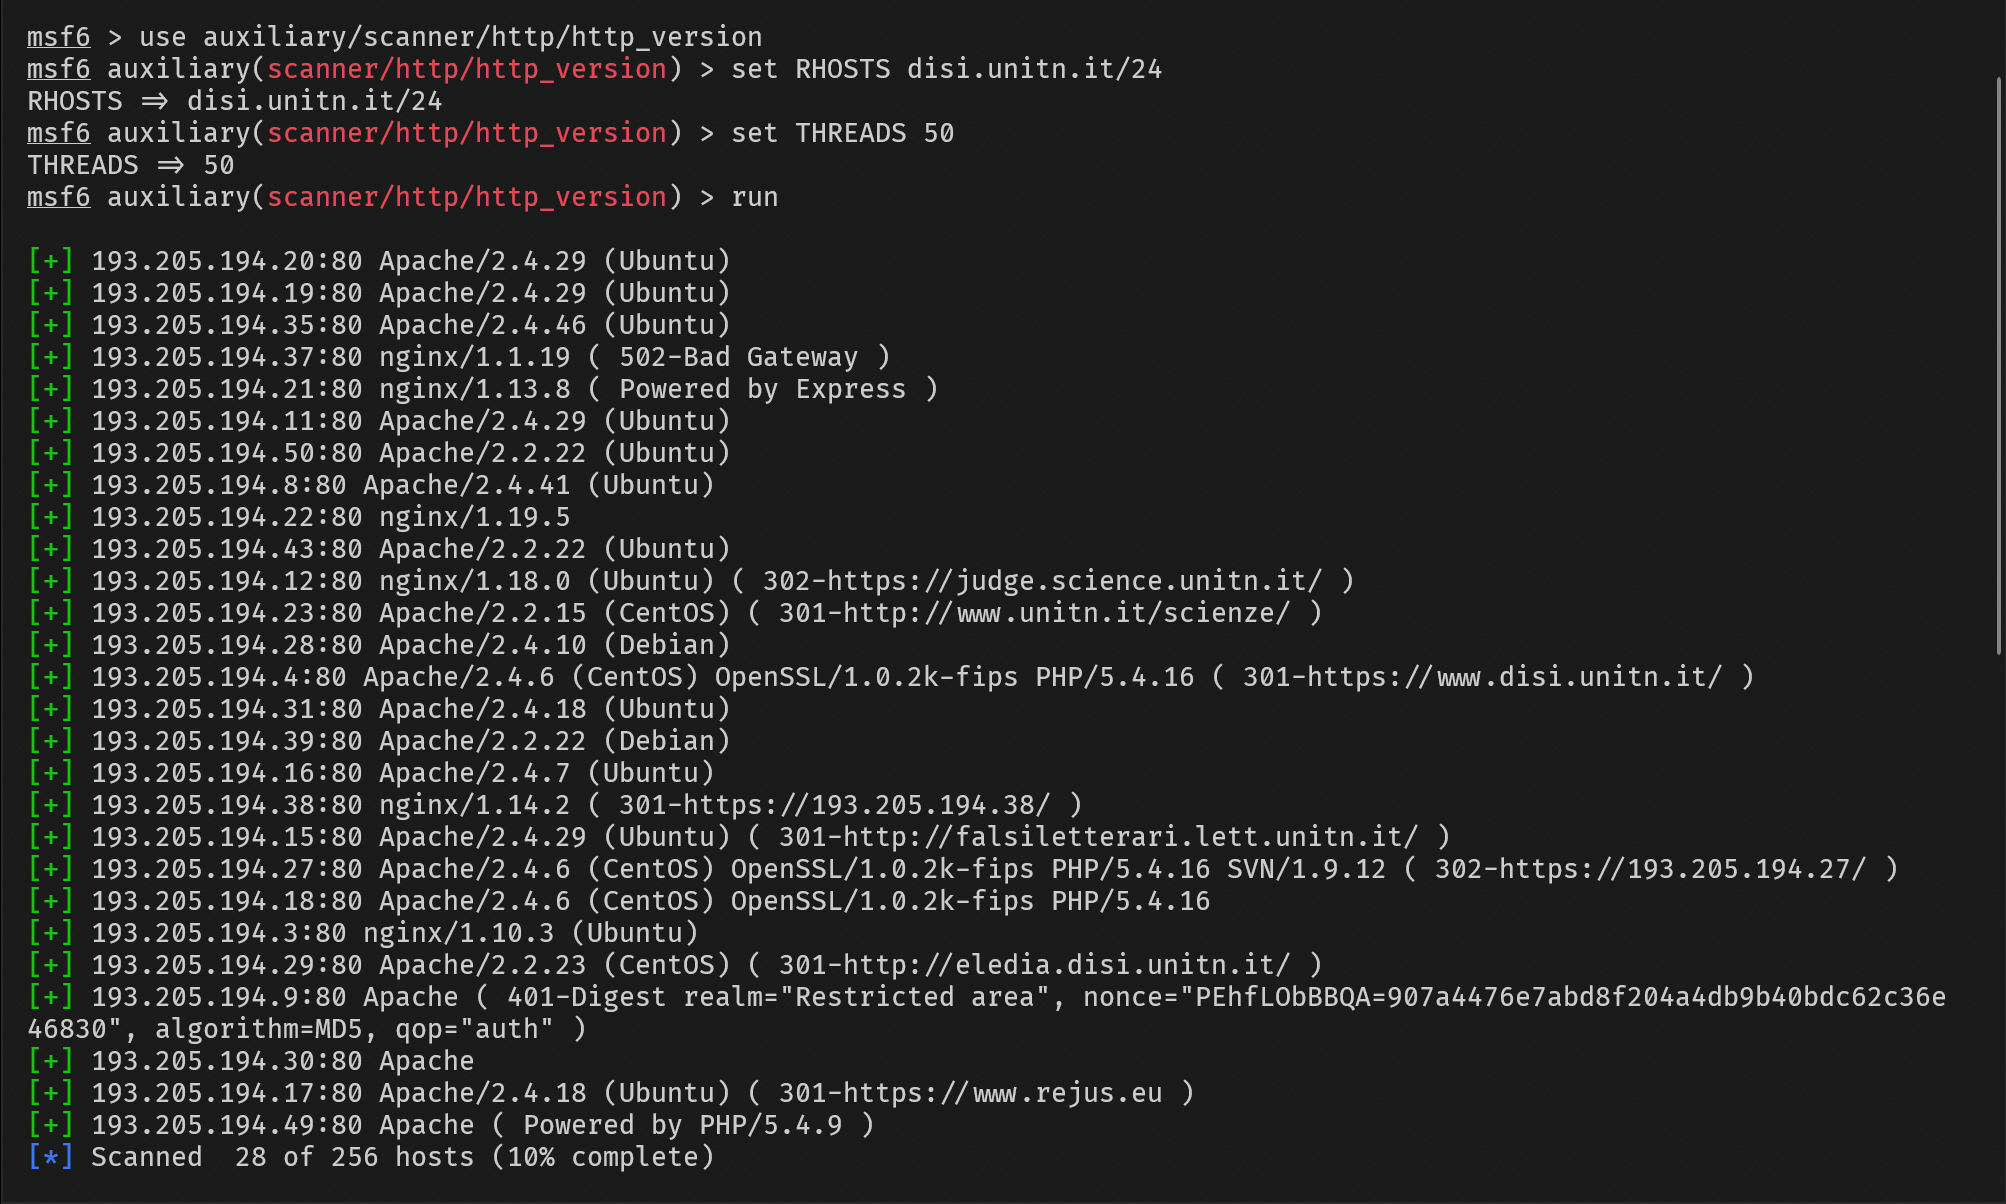
\includegraphics[width=0.85\textwidth]{../drawable/exercise_1_screenshots/es1-http-disi.png}
	\end{figure}
\end{frame}


\subsection{Exercise 2}

% (35)
\begin{frame}
	\frametitle{Exercise 2: Basic Exploits}
	We can now take a first look at Metasploit's exploit modules. We will start by looking at the services offered by the target machine, and exploiting one of them.
\end{frame}

% (36)
\begin{frame}
	\frametitle{Exercise 2: Basic Exploits}
	But before the hacking...databases!
	\begin{figure}
	    \centering
	    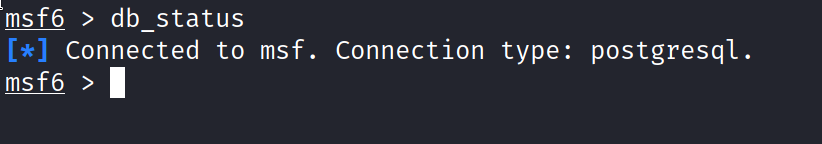
\includegraphics[width=\textwidth]{../drawable/exercise_2_screenshots/db_status.png}
	    \caption{Checking the DB setup is alive and working}
	\end{figure}
\end{frame}

% (37)
\begin{frame}
	\frametitle{Exercise 2: Basic Exploits}
	The DB has been on since we opened the shell. We can check \texttt{services} and \texttt{hosts}.
	
	\begin{figure}
	    \centering
	    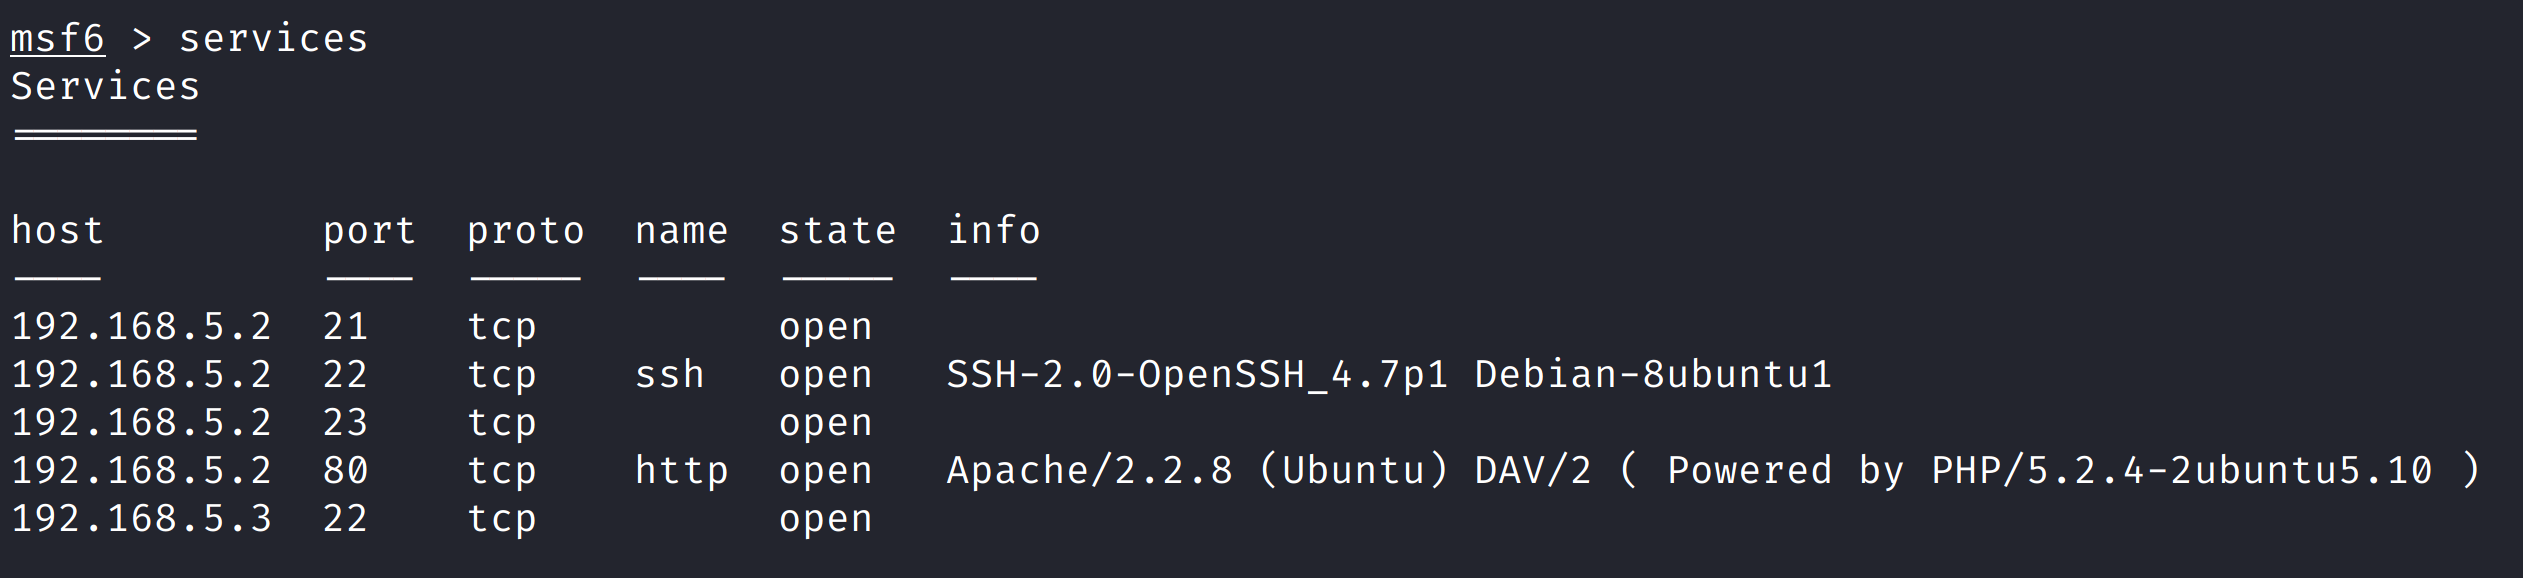
\includegraphics[width=0.75\textwidth]{../drawable/exercise_2_screenshots/services_before.png}
	    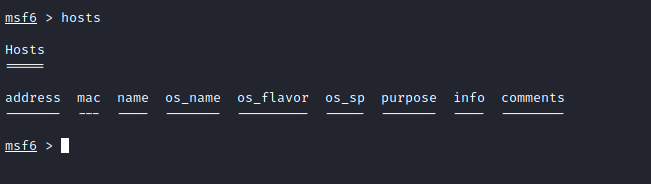
\includegraphics[width=0.75\textwidth]{../drawable/exercise_2_screenshots/hosts_empty.png}
	    \caption{\texttt{services} and \texttt{hosts}}
	\end{figure}
	
	\onslide<2->{
	   If needed, we can wipe data with \texttt{hosts -d} and \texttt{services -d}. However, let's keep it for now.     
	}
\end{frame}

% (38)
\begin{frame}
	\frametitle{Exercise 2: Basic Exploits}
	
	\onslide<1->{
	    Additionally, \texttt{sessions} will still contain previously open \texttt{SSH} connections. Let us terminate them with \texttt{sessions -K}.
	}
	
	\begin{figure}
	    \centering
	    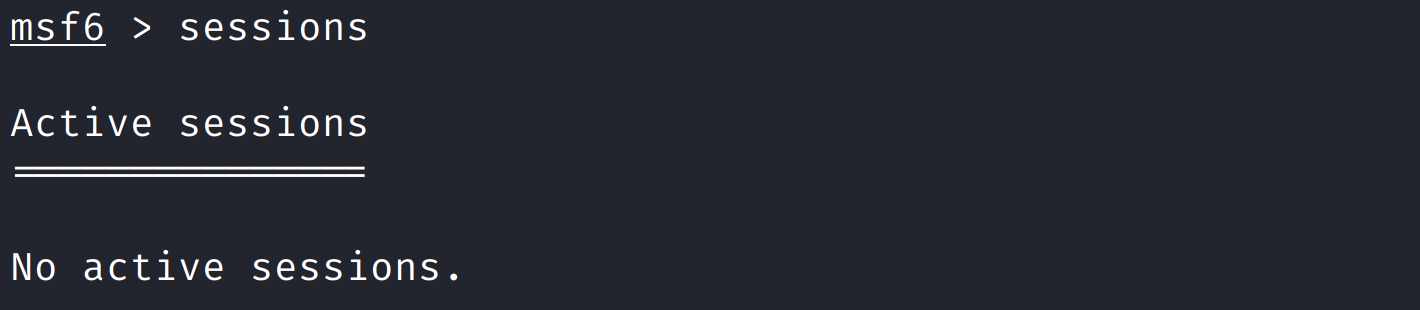
\includegraphics[width=0.7\textwidth]{../drawable/exercise_2_screenshots/sessions_empty.PNG}
	    \caption{\texttt{sessions}}
	\end{figure}
\end{frame}

% (39)
\begin{frame}
	\frametitle{Exercise 2: Basic Exploits}
	% Using \texttt{db\_nmap}:
	\begin{figure}
	    \centering
	    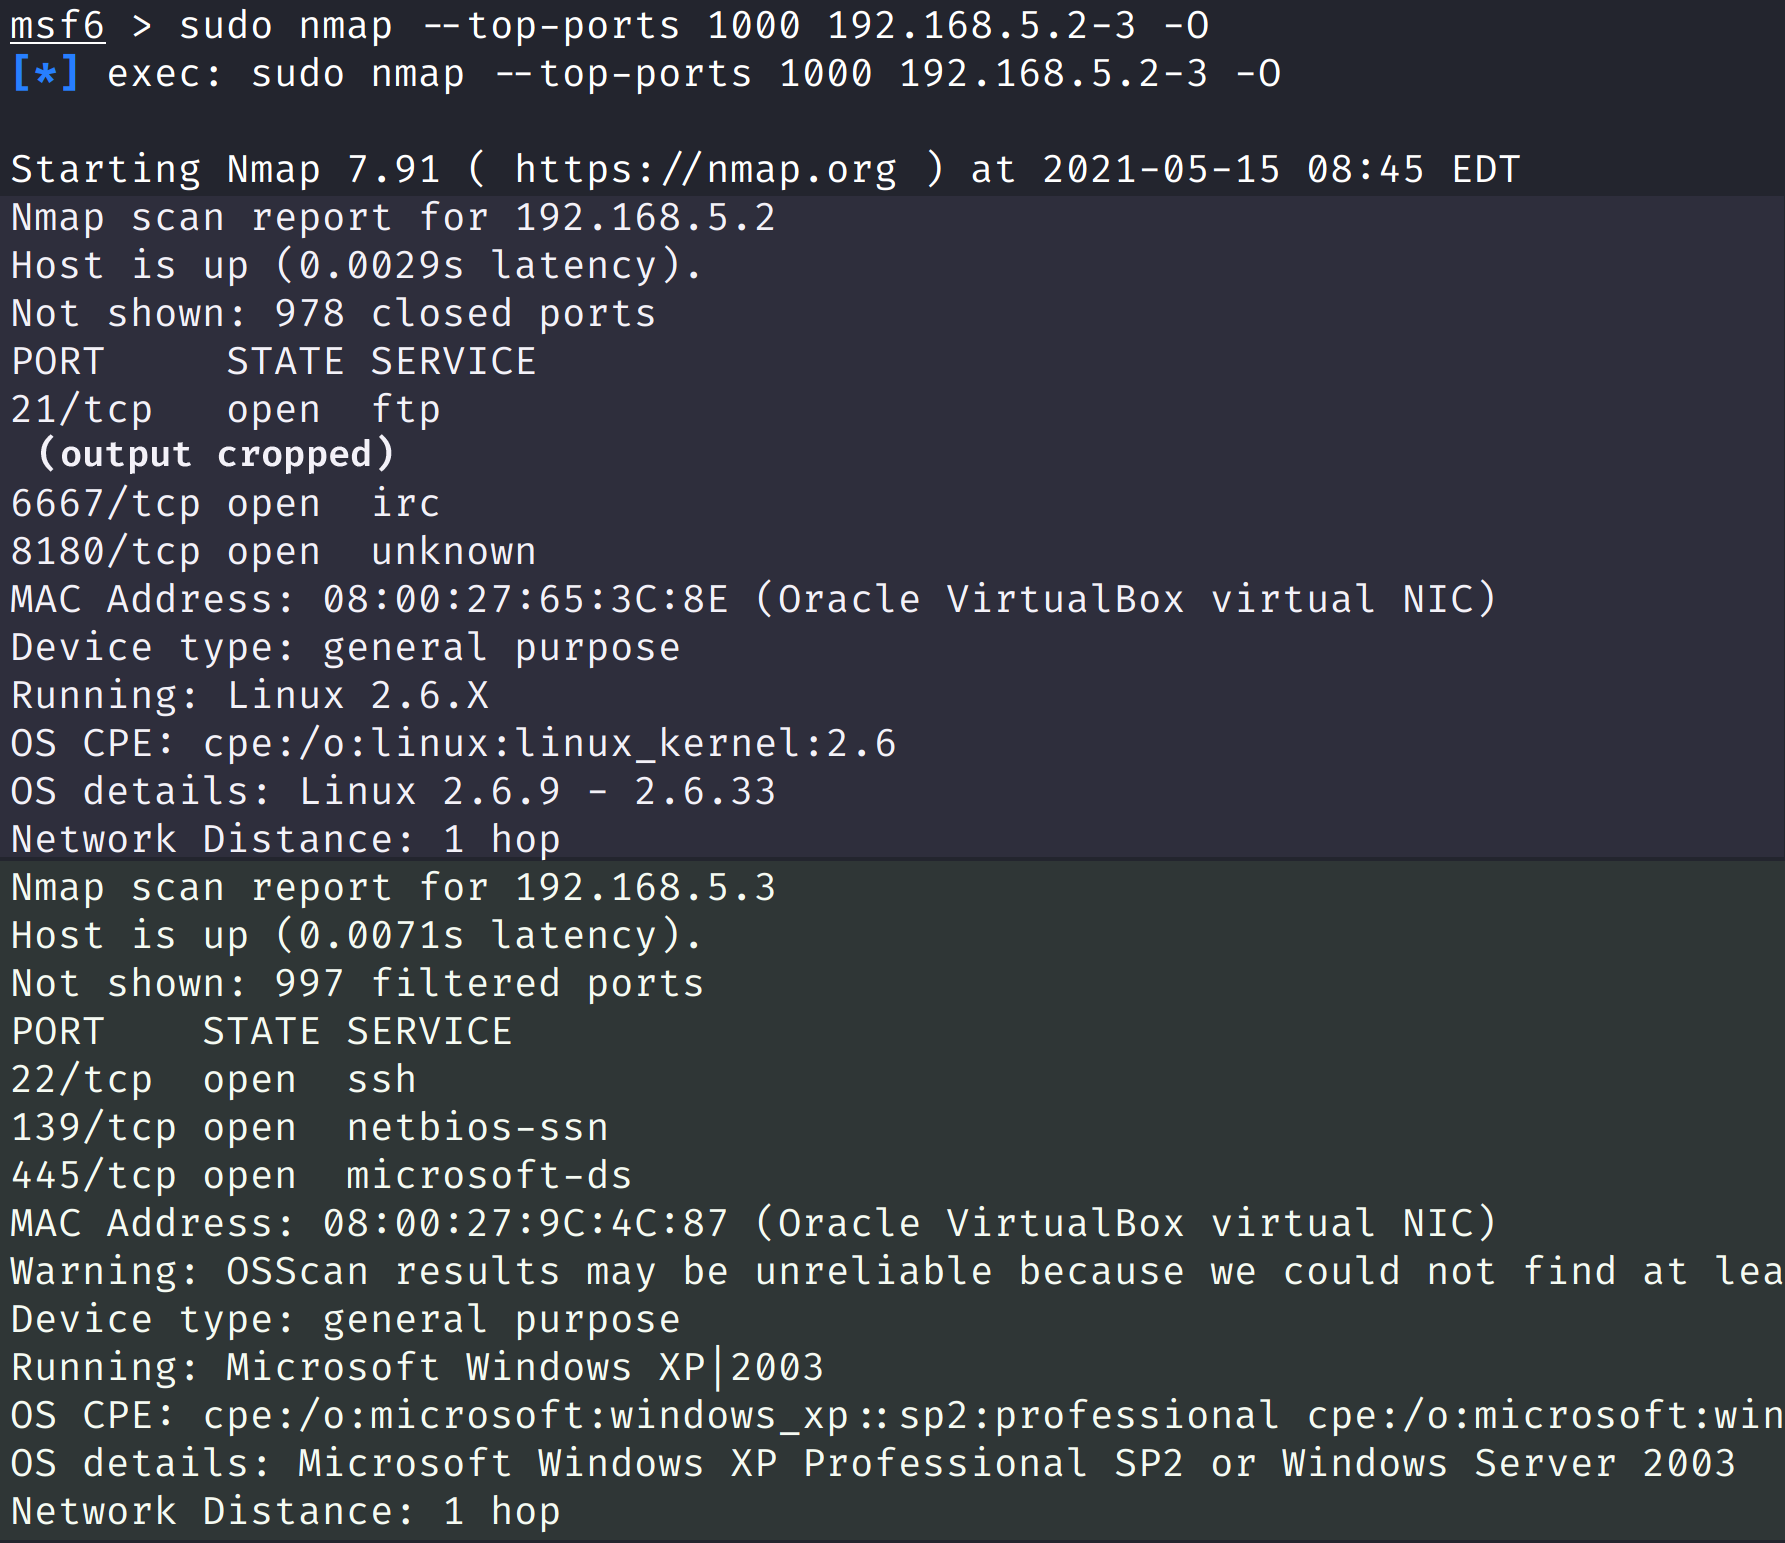
\includegraphics[width=0.96\textheight]{../drawable/exercise_2_screenshots/db_nmap_v2.png}
	    %\caption{Scanning the potential victims (output cropped)}
	\end{figure}
\end{frame}

% (40)
\begin{frame}
	\frametitle{Exercise 2: Basic Exploits}
	Checking the scanned services: now the DB has more entries
	\begin{figure}
	    \centering
	    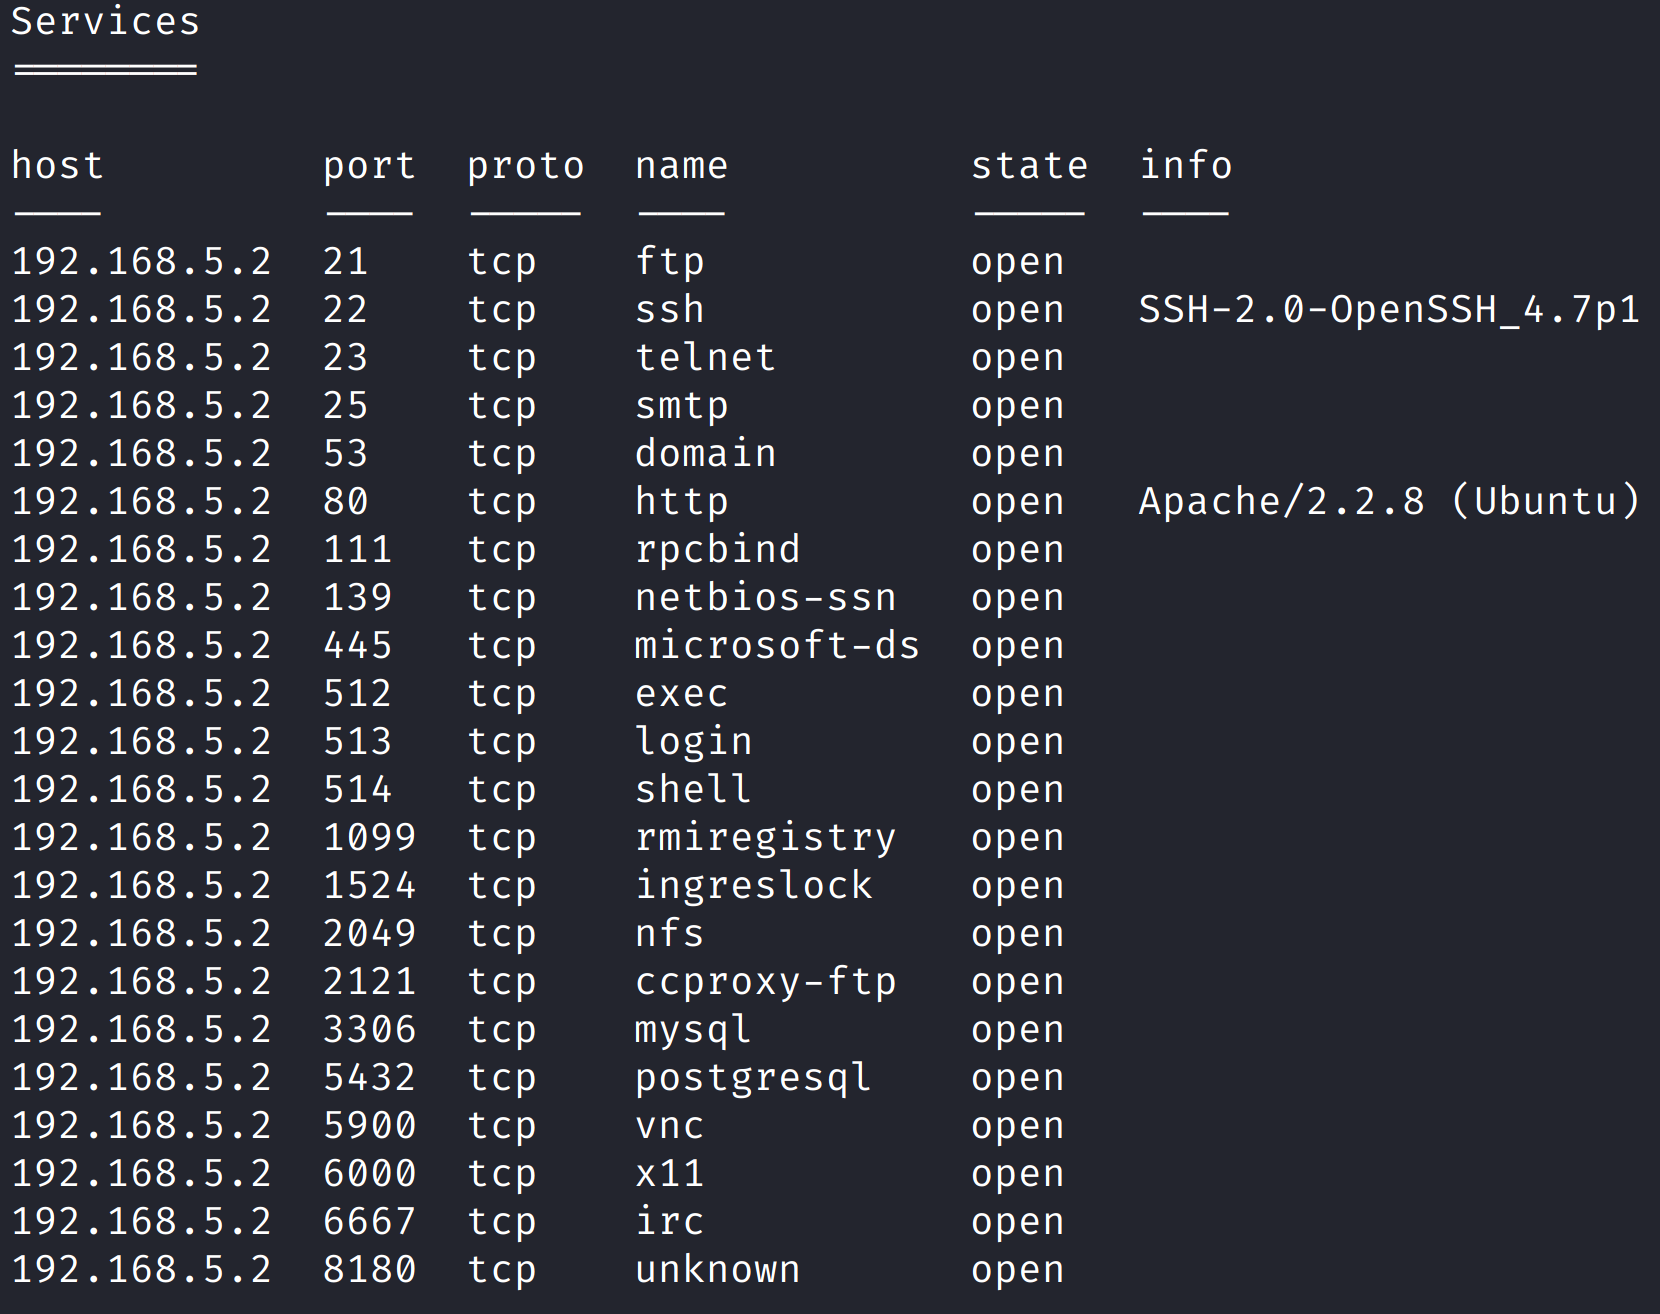
\includegraphics[width=0.6\textwidth]{../drawable/exercise_2_screenshots/services_full_v2.png}
	    \caption{Checking the data that we gathered}
	\end{figure}
\end{frame}

% (40)
%\begin{frame}
%	\frametitle{Exercise 2: Basic Exploits}
%	As we did in the previous exercise, we use a scanner to get some more details on the HTTP service...
%	\begin{figure}
%	    \centering
%	    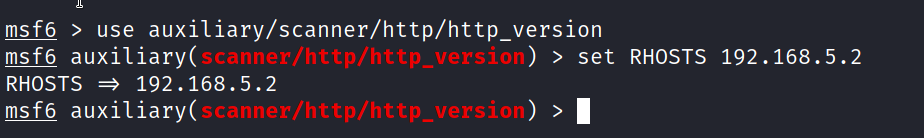
\includegraphics[width=0.8\textwidth]{../drawable/exercise_2_screenshots/use_http_version_scanner.png}
%	    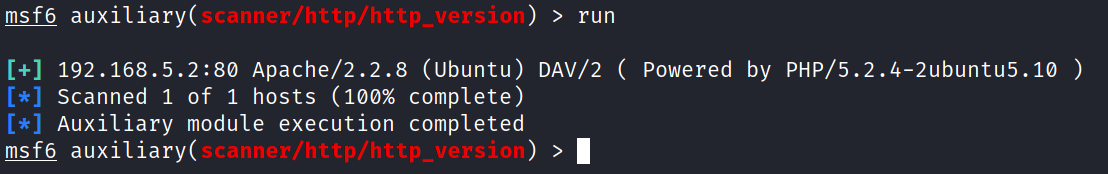
\includegraphics[width=0.8\textwidth]{../drawable/exercise_2_screenshots/execute_http_version.png}
%	    \caption{Preparing the scanner, and then hitting \texttt{run}}
%	\end{figure}
%\end{frame}

% (41)
\begin{frame}
	\frametitle{Exercise 2: Basic Exploits}
	In the previous exercise, we discovered that the host is running Apache with an old version of \texttt{PHP} (\texttt{services}). We can take advantage of that:
	\begin{figure}
	    \centering
	    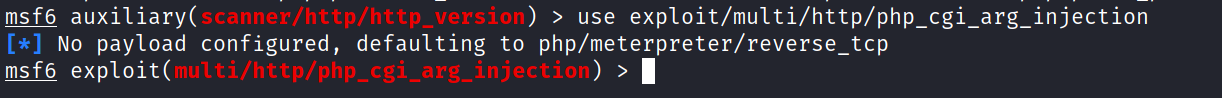
\includegraphics[width=0.9\textwidth]{../drawable/exercise_2_screenshots/use_exploit_cgi_exception.png}
	    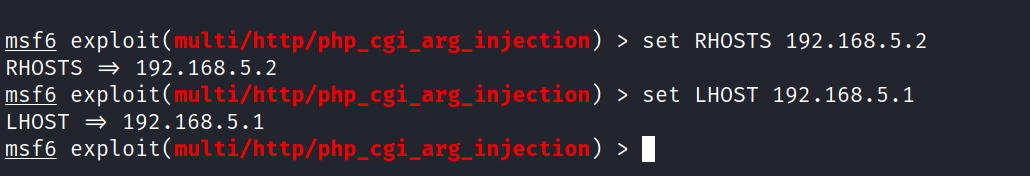
\includegraphics[width=0.9\textwidth]{../drawable/exercise_2_screenshots/set_exploit_options.png}
	    \caption{Using the default payload and setting options}
	\end{figure}
\end{frame}

% (42)
\begin{frame}
	\frametitle{Exercise 2: Basic Exploits}
    And now we have a reverse shell with Meterpreter:
	\begin{figure}
	    \centering
        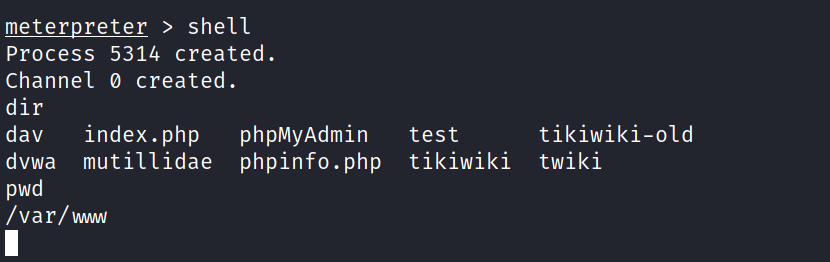
\includegraphics[width=\textwidth]{../drawable/exercise_2_screenshots/shell_opened.png}
	    \caption{Opening a shell with Meterpreter}
	\end{figure}
\end{frame}

% (43)
\begin{frame}
	\frametitle{Exercise 2: Exploit details}
    The exploit we used has CVE-ID \texttt{CVE-2012-1823}:
    \begin{block}{CVE-2012-1823}
        \texttt{sapi/cgi/cgi\_main.c} in \texttt{PHP} before 5.3.12 and 5.4.x before 5.4.2, when configured as a CGI script (aka php\-cgi), does not properly handle query strings that lack an = (equals sign) character, which allows remote attackers to execute arbitrary code by placing command-line options in the query string, related to lack of skipping a certain php\_getopt for the 'd' case.      
    \end{block}
\end{frame}

% (44)
\begin{frame}[fragile]
	\frametitle{Exercise 2: Exploit details}
	The source of the buffer overflow in \texttt{cgi\_main.c}
    \begin{lstlisting}[showspaces=false,breaklines=true]
// [...] here len is the same length of php_optarg
memcpy(
    cgi_sapi_module.ini_entries + ini_entries_len,
    php_optarg,
    len
);
// [...]
    \end{lstlisting}
\end{frame}

% (45)
\begin{frame}[fragile]
	\frametitle{Exercise 2: Exploit details}
	Snippet from the exploit file
    \begin{lstlisting}[showspaces=false,breaklines=true,showstringspaces=false]
payload_oneline = "<?php " + payload.encoded.gsub(/\s*#.*$/, "").gsub("\n", "")
response = send_request_cgi( {
    'method' => "POST",
    'global' => true,
    'uri'    => "#{uri}?#{qs}",
    'data'   => payload_oneline,
}, 0.5)
    \end{lstlisting}
\end{frame}

% (46)
\begin{frame}
	\frametitle{Exercise 2: Reverse shells}
    The payload was a \emph{reverse shell}...what does it mean?
	\begin{figure}
	    \centering
        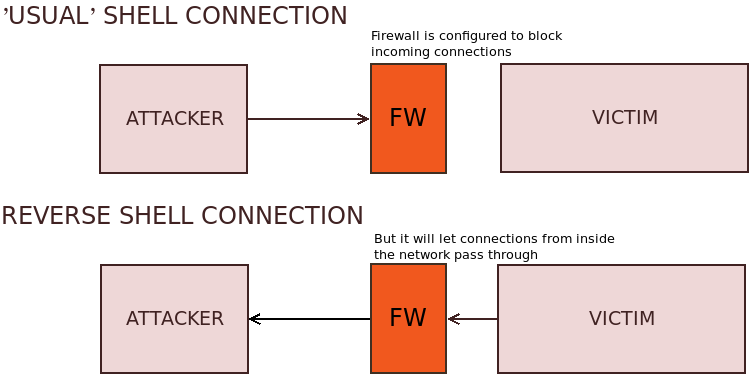
\includegraphics[width=0.8\textwidth]{../drawable/decorations/schema_reverse_shell.png}
	    \caption{Shell and reverse shell connections}
	\end{figure}
\end{frame}

\subsection{Exercise 3}

% (47)
\begin{frame}
	\frametitle{Exercise 3: Infected PDF}
	Now we're going to generate an infected \texttt{PDF} file, to use as an attack vector towards a Windows XP VM.
\end{frame}

% (48)
\begin{frame}
    \frametitle{Exercise 3: Infected PDF}
    \begin{figure}
        \centering
        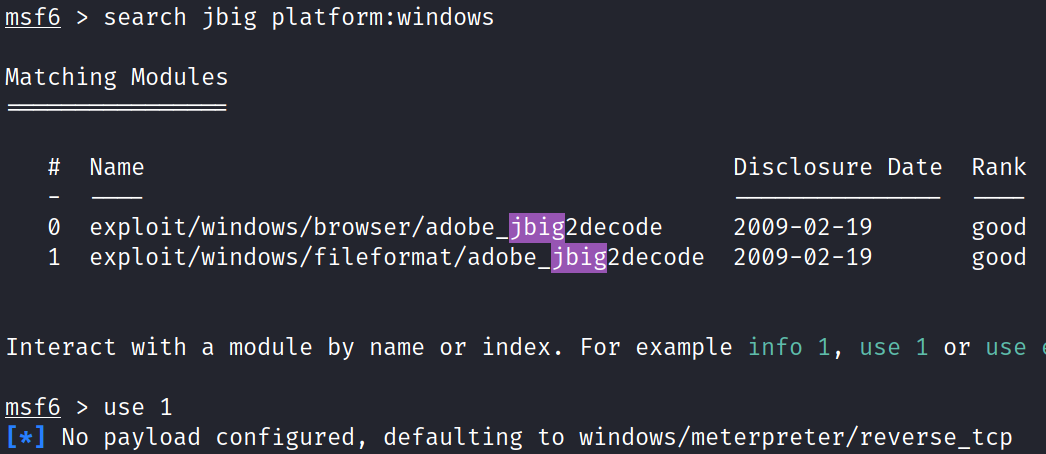
\includegraphics[width=\textwidth]{../drawable/exercise_3_screenshots/module_selection.png}
        \caption{Selecting the exploit to use}
    \end{figure}
\end{frame}

% (49)
\begin{frame}
    \frametitle{Exercise 3: Infected PDF}
    \begin{figure}
        \centering
        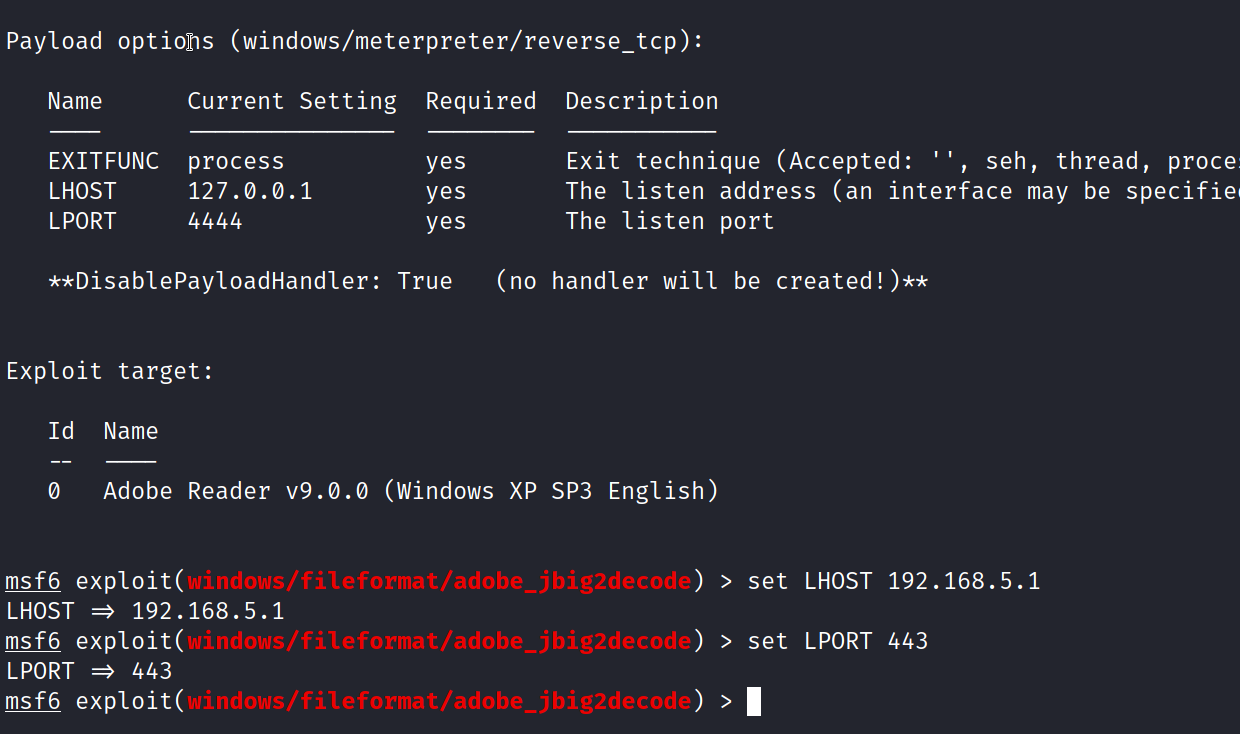
\includegraphics[width=0.8\textwidth]{../drawable/exercise_3_screenshots/module_set_options.png}
        \caption{Setting the options}
    \end{figure}
\end{frame}

% (50)
\begin{frame}
    \frametitle{Exercise 3: Infected PDF}
    \begin{figure}
        \centering
        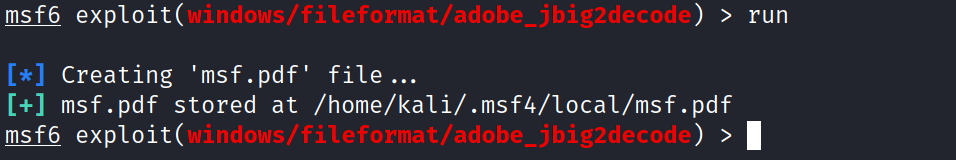
\includegraphics[width=\textwidth]{../drawable/exercise_3_screenshots/run_exploit.png}
        \caption{Generating the infected file}
    \end{figure}
\end{frame}

% (51)
\begin{frame}
    \frametitle{Exercise 3: Infected PDF}
    \begin{figure}
        \centering
        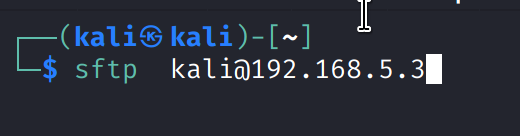
\includegraphics[width=\textwidth]{../drawable/exercise_3_screenshots/sftp_infected_file.png}
        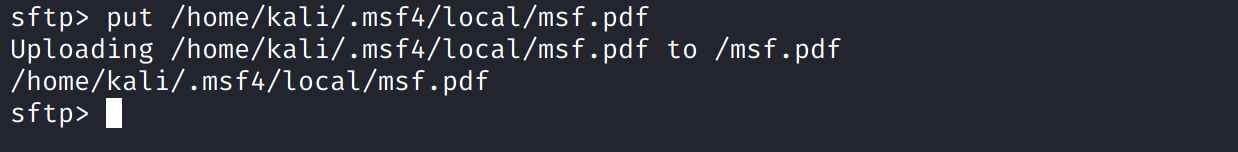
\includegraphics[width=\textwidth]{../drawable/exercise_3_screenshots/put_completed.png}
        \caption{Sending the file to our Windows XP VM}
    \end{figure}
\end{frame}

% (52)
\begin{frame}
    \frametitle{Exercise 3: Infected PDF}
    \begin{figure}
        \centering
        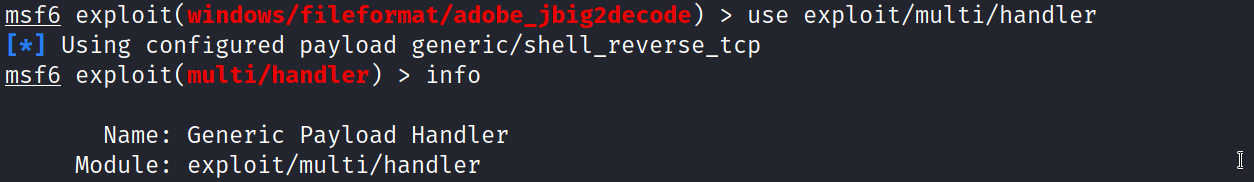
\includegraphics[width=0.92\textwidth]{../drawable/exercise_3_screenshots/generic_payload_handler.png}
        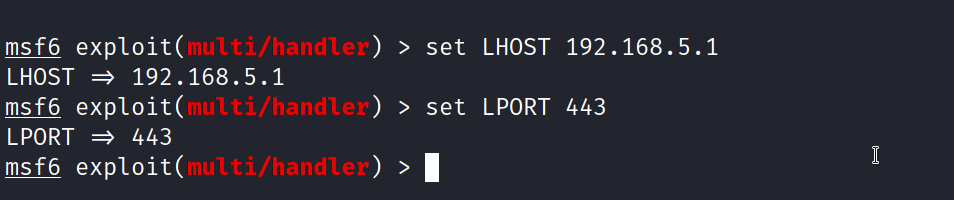
\includegraphics[width=0.92\textwidth]{../drawable/exercise_3_screenshots/set_handler_parameters.png}
        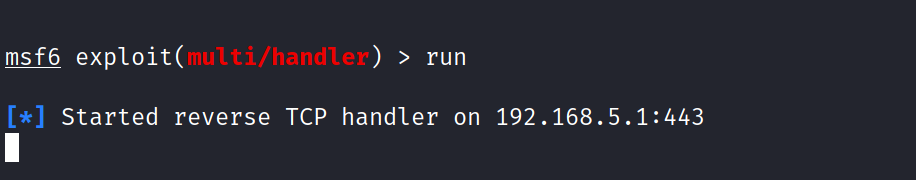
\includegraphics[width=0.92\textwidth]{../drawable/exercise_3_screenshots/handler_listening.png}
        \caption{Starting the reverse shell handler}
    \end{figure}
\end{frame}

% (53)
\begin{frame}
    \frametitle{Exercise 3: Infected PDF}
    \begin{figure}
        \centering
        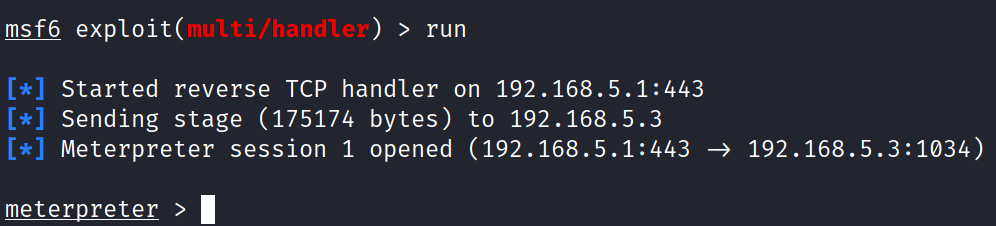
\includegraphics[width=\textwidth]{../drawable/exercise_3_screenshots/meterpreter_opened.png}
        \caption{Reverse shell managed to reach the attacker}
    \end{figure}
\end{frame}

% (54)
\begin{frame}
    \frametitle{Exercise 3: Infected PDF}
    \begin{figure}
        \centering
        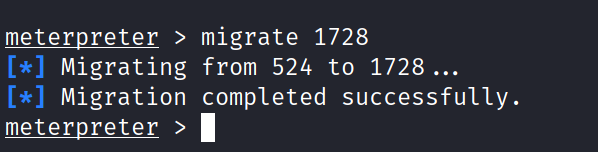
\includegraphics[width=0.95\textwidth]{../drawable/exercise_3_screenshots/meterpreter_migration.png}
        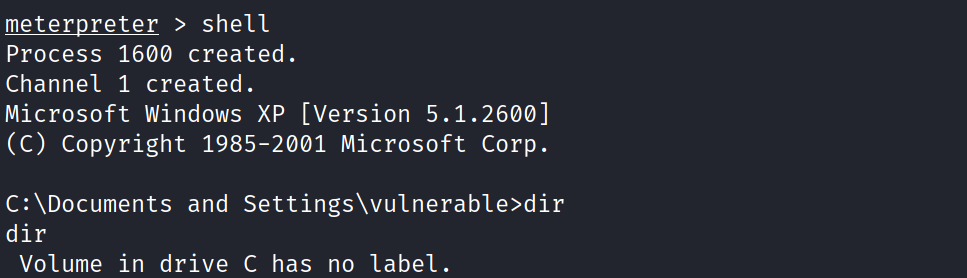
\includegraphics[width=0.95\textwidth]{../drawable/exercise_3_screenshots/meterpreter_shell_opened_cropped.png}
        \caption{Migrating shell code to another process}
    \end{figure}
\end{frame}

% (56)
\begin{frame}
    \frametitle{Exercise 3}
    \begin{figure}
        \centering
        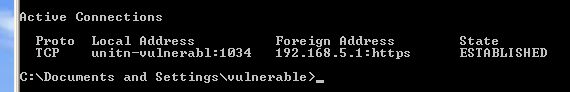
\includegraphics[width=\textwidth]{../drawable/exercise_3_screenshots/victim_connection.PNG}
        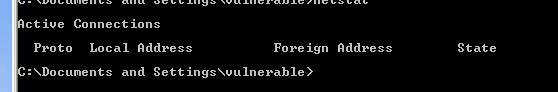
\includegraphics[width=\textwidth]{../drawable/exercise_3_screenshots/victim_connections_after_exit.PNG}
        \caption{Connections active on the victim, during and after the attack}
    \end{figure}
\end{frame}

% (56)
\begin{frame}
    \frametitle{Exercise 3: Exploit details}
    \begin{block}{CVE-2009-0658}
        Buffer overflow in Adobe Reader 9.0 and earlier, and Acrobat 9.0 and earlier, allows remote attackers to execute arbitrary code via a crafted PDF document, related to a non-JavaScript function call and possibly an embedded JBIG2 image stream, as exploited in the wild in February 2009 by \texttt{Trojan.Pidief.E}.
    \end{block}
\end{frame}

% (57)
\section{Conclusion}

% (58)
\begin{frame}
    \frametitle{Wrapping up}
    \onslide<1-> {
        What we showed in this lab is just about barely scratching the surface of the capabilities of Metasploit.
    }
    
    \medskip
    
    \onslide<2->{
        In the following lab, you'll be able to have a grasp on more advanced topics, such as \texttt{msfvenom}, and experiment with more complicated exploits and different OSs.
    }
\end{frame}

% (59)
\begin{frame}
    \frametitle{Wrapping up}
    Thank you for your kind attention!
            
    \begin{figure}
        \centering
        
\includegraphics[width=0.7\textwidth]{../drawable/decorations/image-thatsall.jpg}
    \end{figure}
\end{frame}


%\frame{\titlepage}

\end{document}
